\part{三角形五心}
\section{外心}

\begin{definition}[外心]
    三角形外接圆的圆心简称为三角形的外心,通常使用O表示。
\end{definition}

\begin{figure}[H]
    \centering
    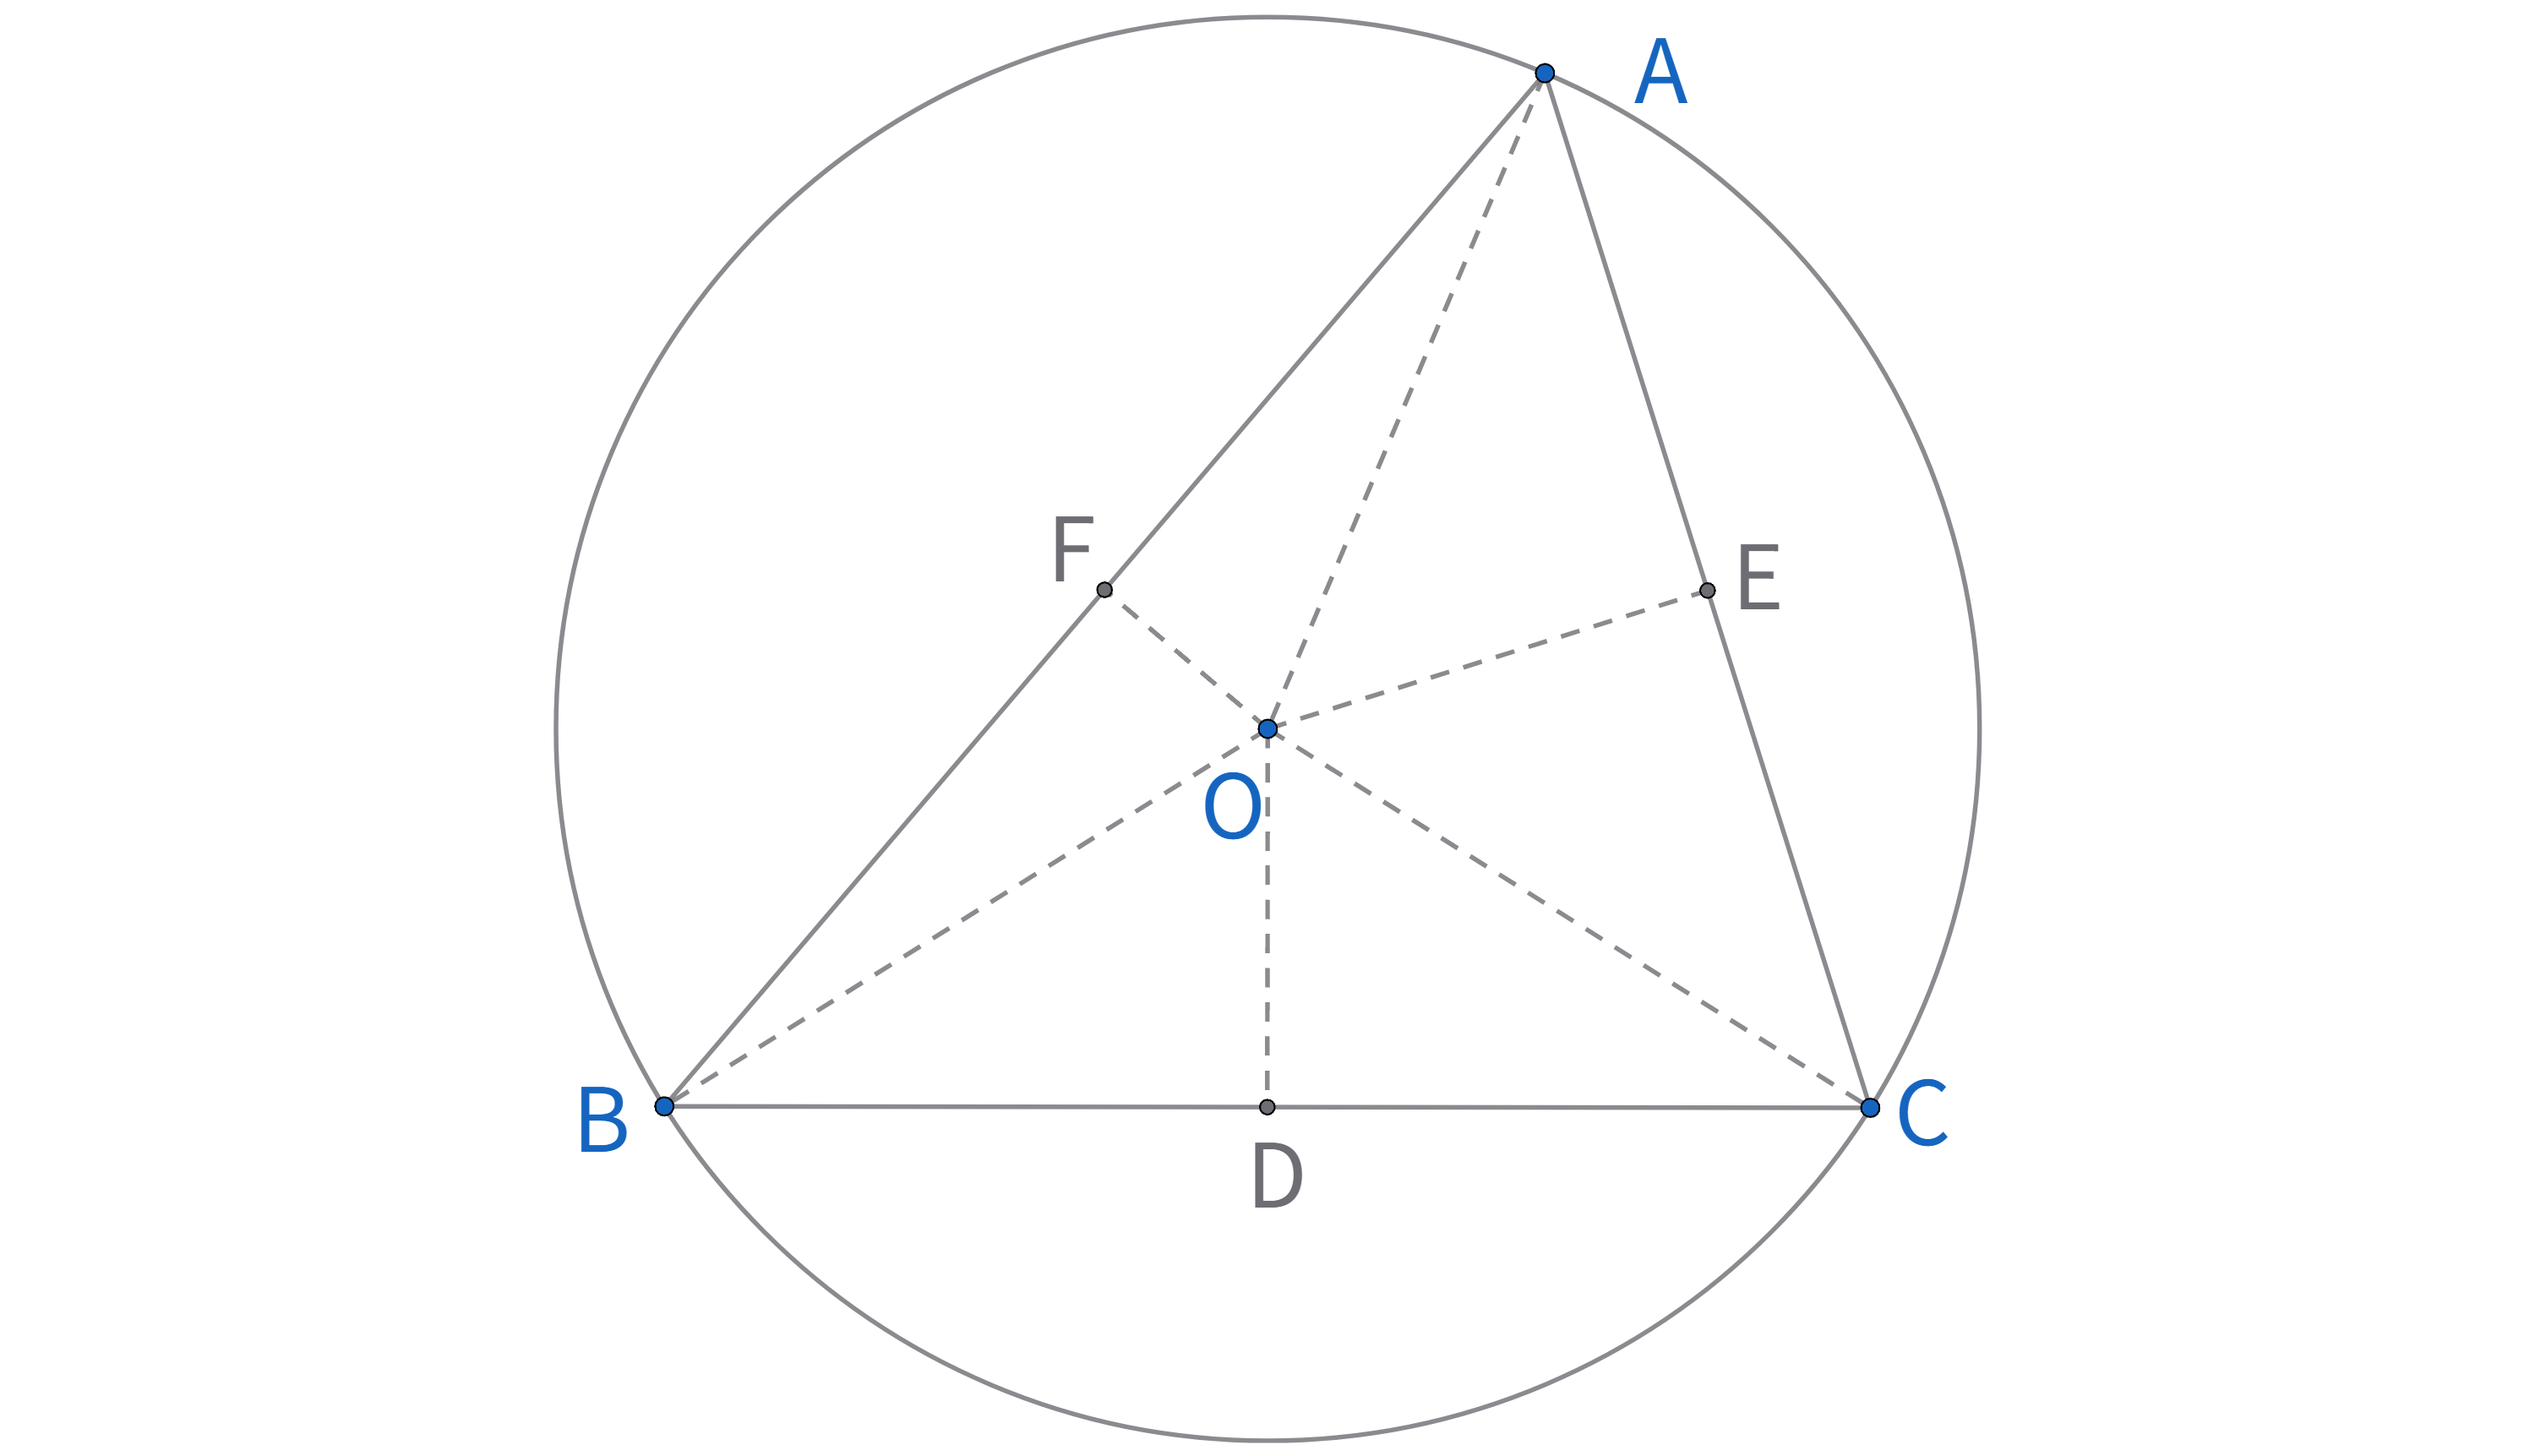
\includegraphics[width=0.8\linewidth]{figures/三角形五心/外心.png}
    \caption{外心}
\end{figure}

\begin{proposition}[外心性质]
    三角形外心具有如下性质。
    
    (1) 三角形的外心是三条边中垂线的交点。

    (2) 平面内一点是三角形外心的充分必要条件为:该点到三顶点的距离相等。

    (3) 锐角三角形的外心在形内,直角三角形的外心为斜边中点,钝角三角形的外心在形外。
\end{proposition}

\begin{exercise}
    用$\triangle ABC$外接圆半径长$R$以及三顶角的正弦函数表示所有线段长。
\end{exercise}


%--------------------------------------------------------------
\newpage 
\section{内心}

\begin{definition}[内心]
    三角形内切圆的圆心简称为三角形的内心,通常使用I表示。
\end{definition}

\begin{figure}[H]
    \centering
    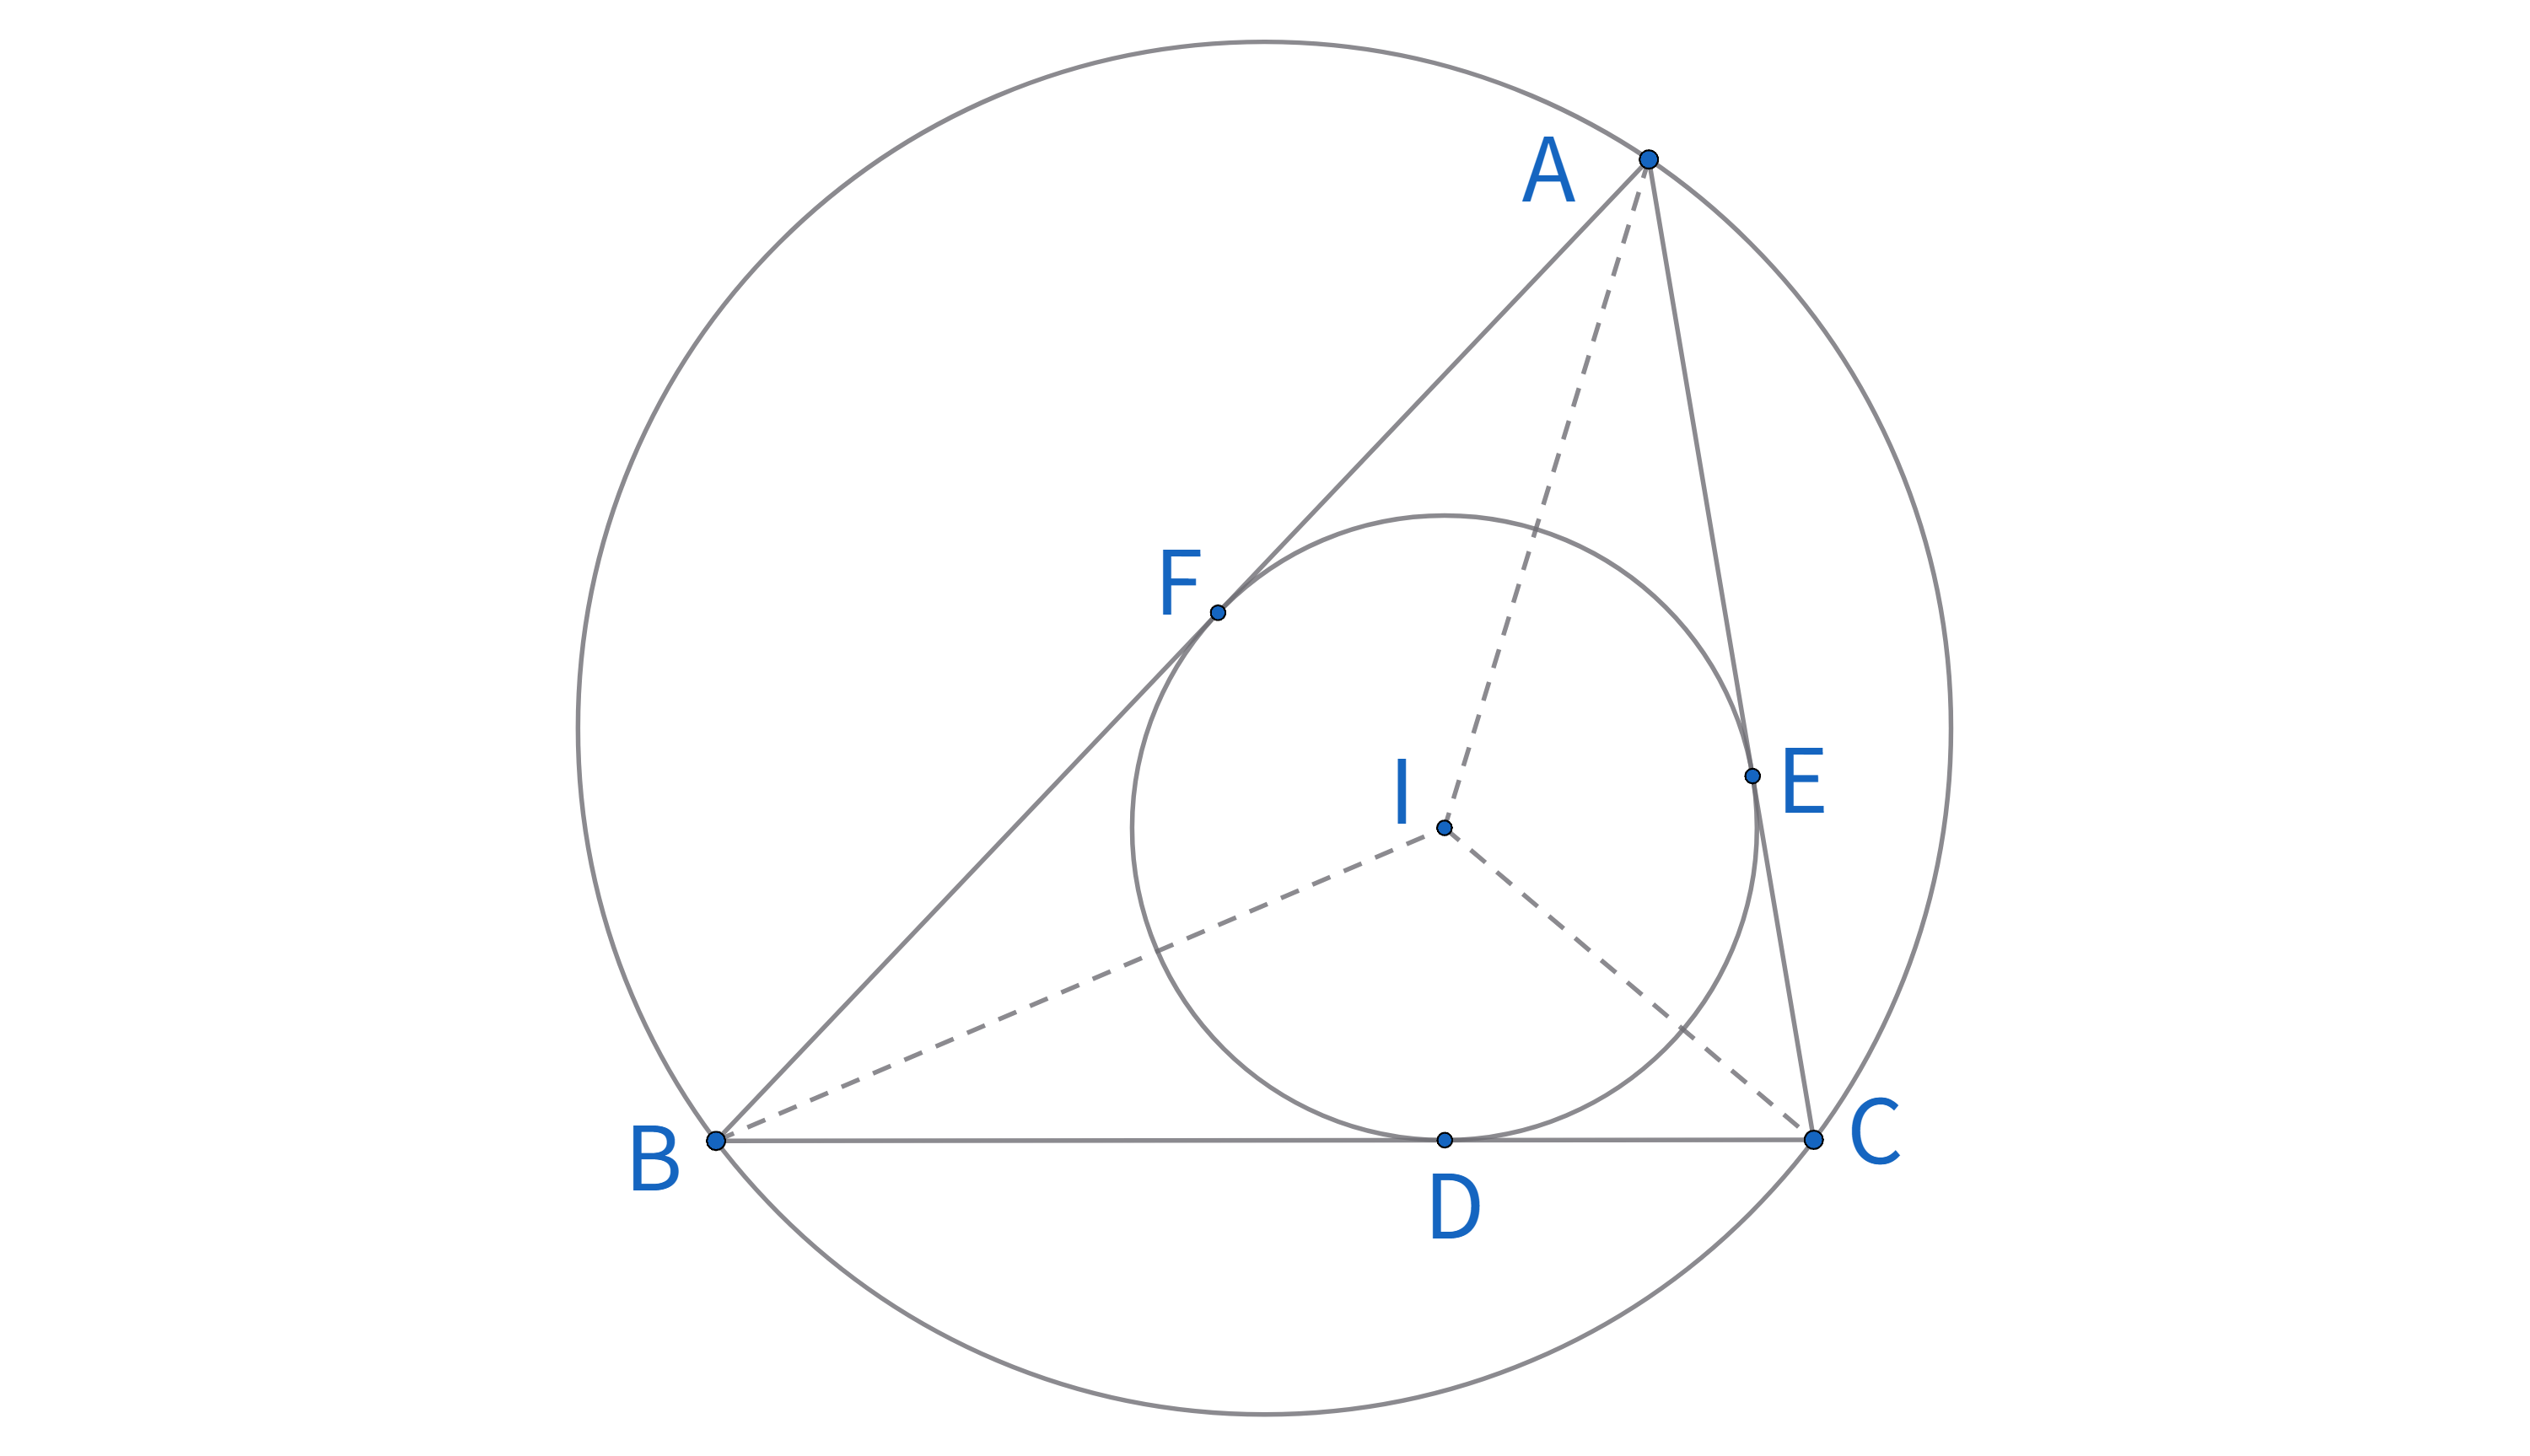
\includegraphics[width=0.8\linewidth]{figures/三角形五心/内心.png}
    \caption{内心}
\end{figure}

\begin{proposition}[内心性质]
    三角形内心具有如下性质。
    
    (1) 三角形的内心是三条内角平分线的交点。

    (2) 内心到三边的距离相等。

    (3) 平面内一点I是三角形$\triangle ABC$内心的充分必要条件为:
    $$\angle BIC = 90^\circ +\frac{1}{2}A,\quad \angle AIC = 90^\circ +\frac{1}{2}B,
    \quad \angle AIB =90^\circ +\frac{1}{2}C.$$

\end{proposition}


\begin{proposition}[切线长性质]
    设D、E、F分别为内切圆I在BC、CA、AB上的切点,则
    $$
    \begin{aligned}
    AE&=AF=s-a = \frac{1}{2}(b+c - a),\\
    BF&=BD=s - b =\frac{1}{2}(a+c - b),\\
    CD&=CE=s - c= \frac{1}{2}(a+b - c).
    \end{aligned}
    $$
\end{proposition}



\newpage 
\begin{theorem}[鸡爪定理]
    对平面内任意$\triangle ABC$,O、I分别为其外心和内心。设AI延长线与圆O相交于D,
    D为$\overset{{\frown}}{BC}$的中点,并且满足
    $$DB=DI=DC.$$
\end{theorem}

\begin{figure}[H]
    \centering
    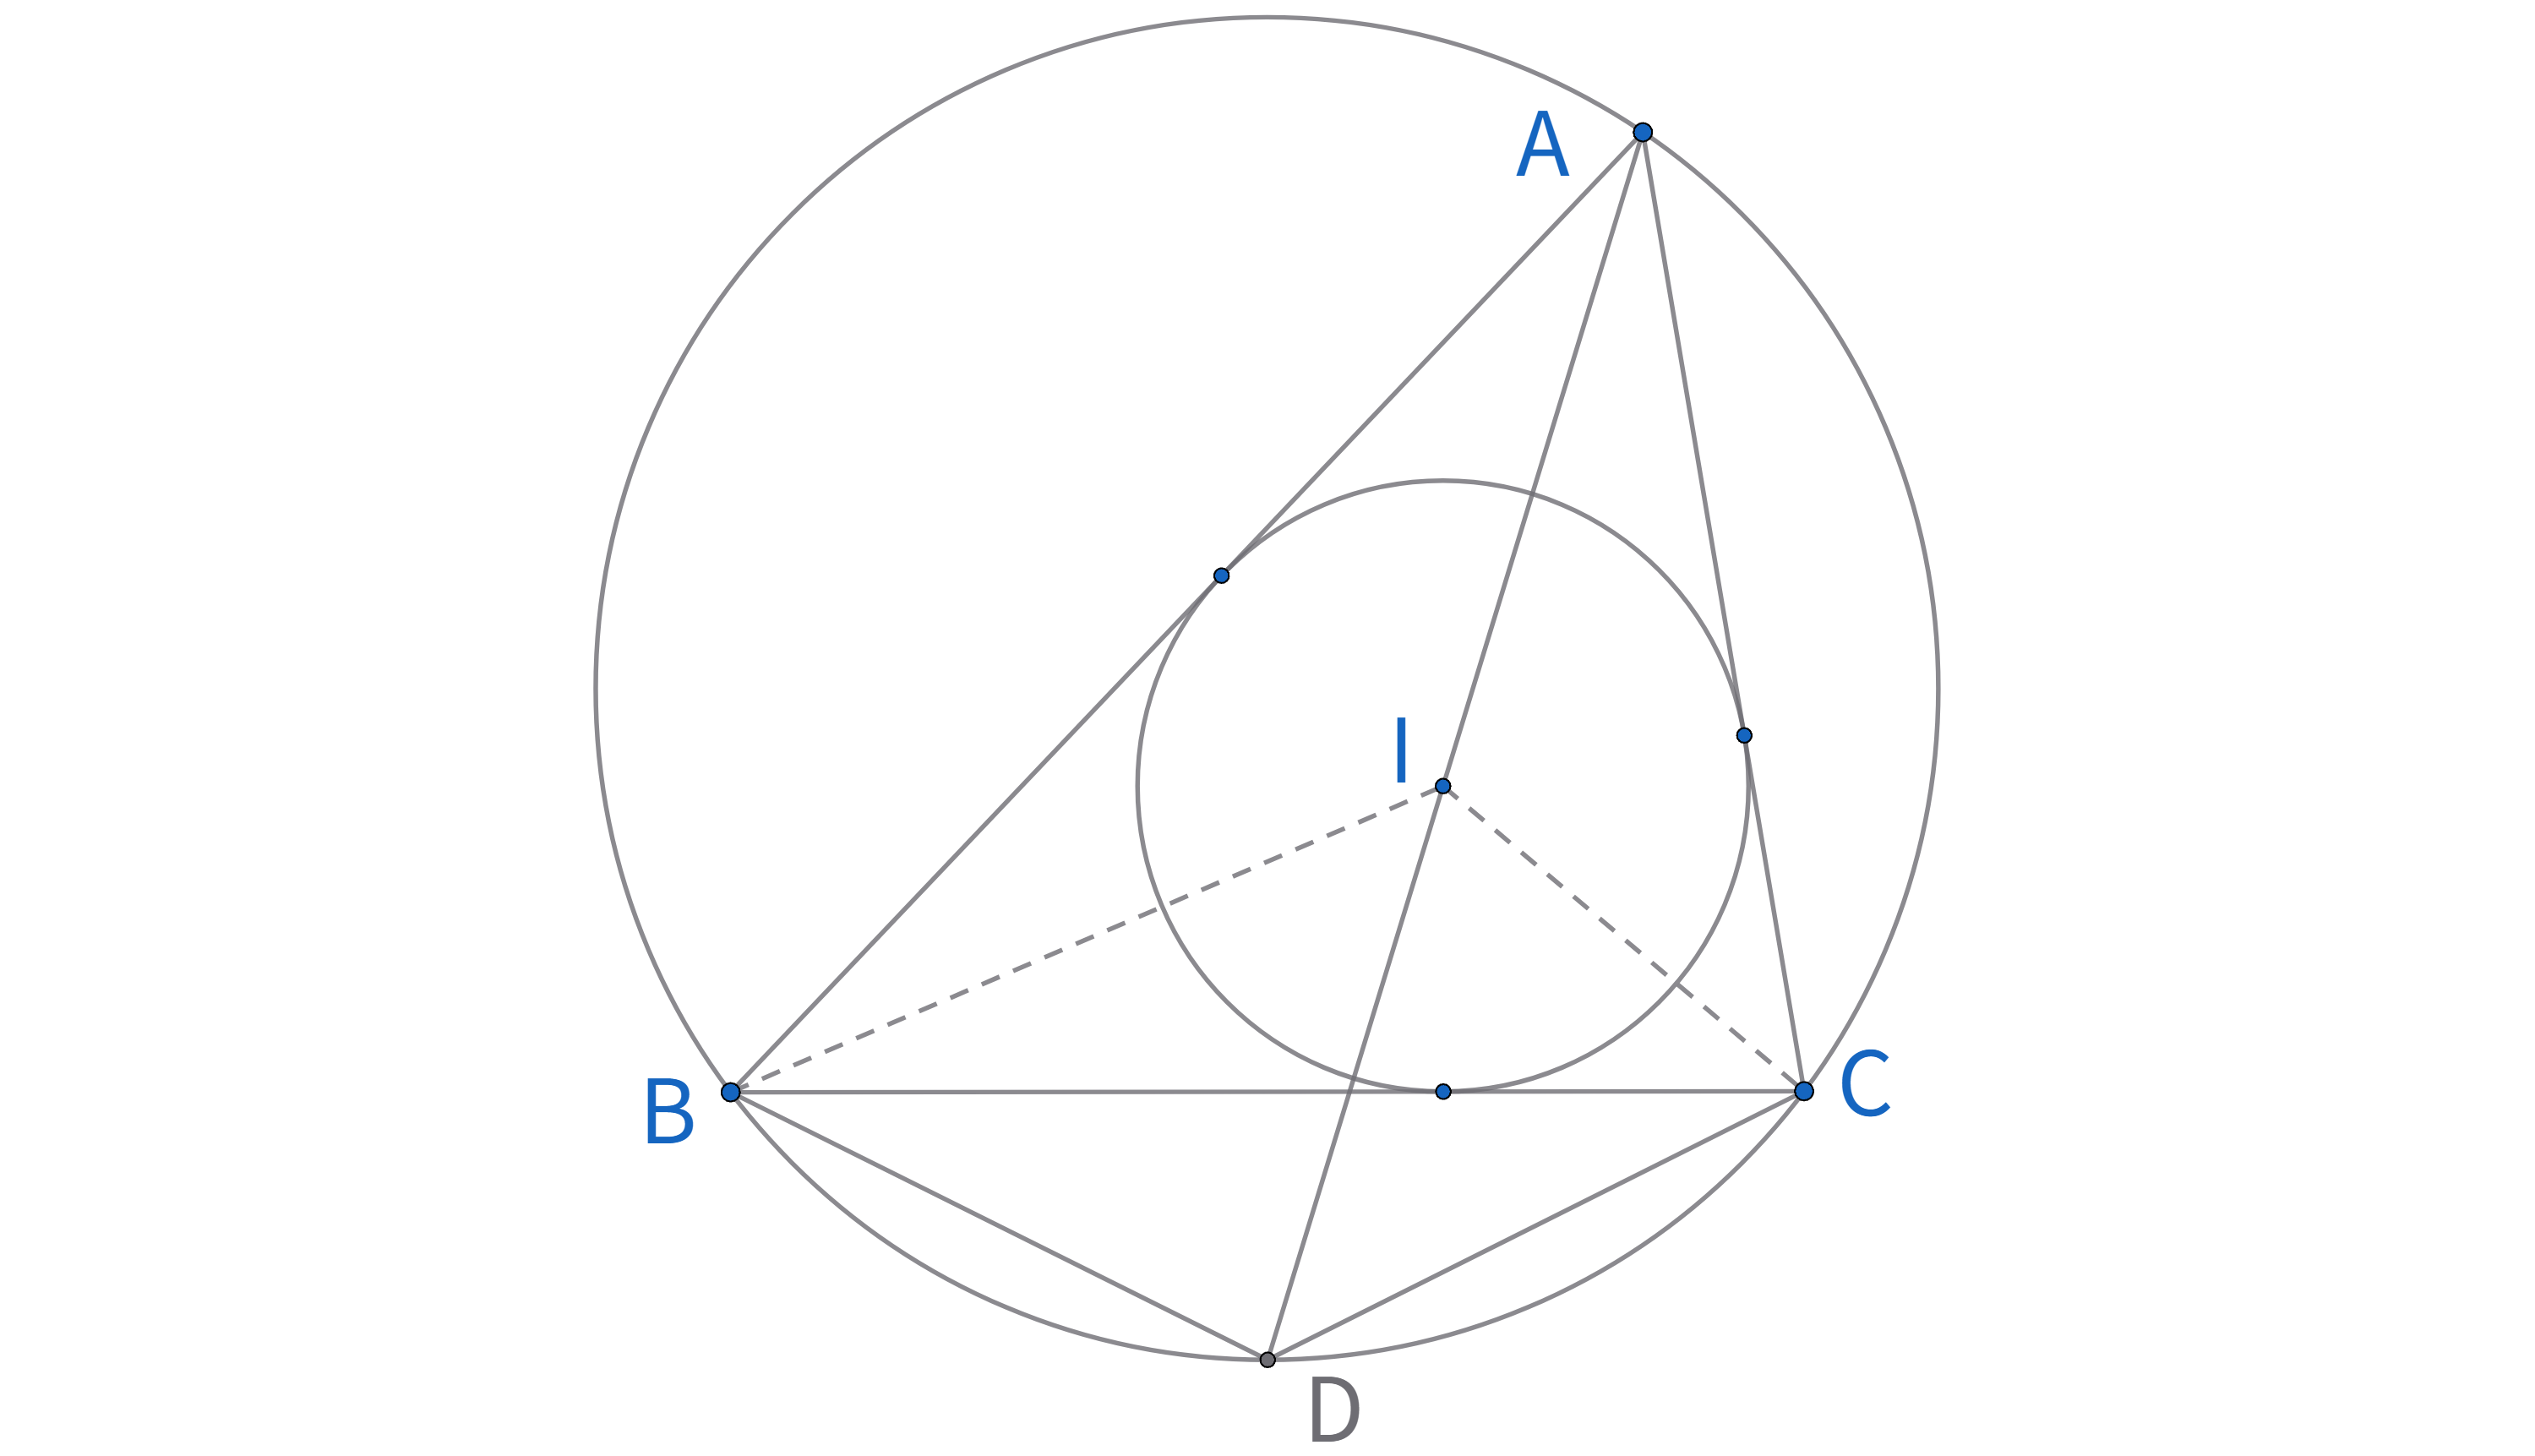
\includegraphics[width=0.8\linewidth]{figures/三角形五心/鸡爪定理.png}
    \caption{鸡爪定理}
\end{figure}

\begin{exercise}
    计算$\angle IBD, \angle ICD, \angle BID, \angle CID$。
\end{exercise}
\begin{exercise}
    表示$\triangle ABC$内切圆半径长。
\end{exercise}
\begin{exercise}
    设$\triangle DEF$为切点三角形,表示$\triangle DEF$的三边长和三顶角大小。
\end{exercise}
\begin{exercise}[内外径的欧拉定理]
    $\triangle ABC$的外接圆半径和内切圆半径分别为$R,r.$ 若$O,I$分别是二者的圆心,则$OI^2 = R(R-2r).$
\end{exercise}


% \begin{figure}[H]
%     \centering
%     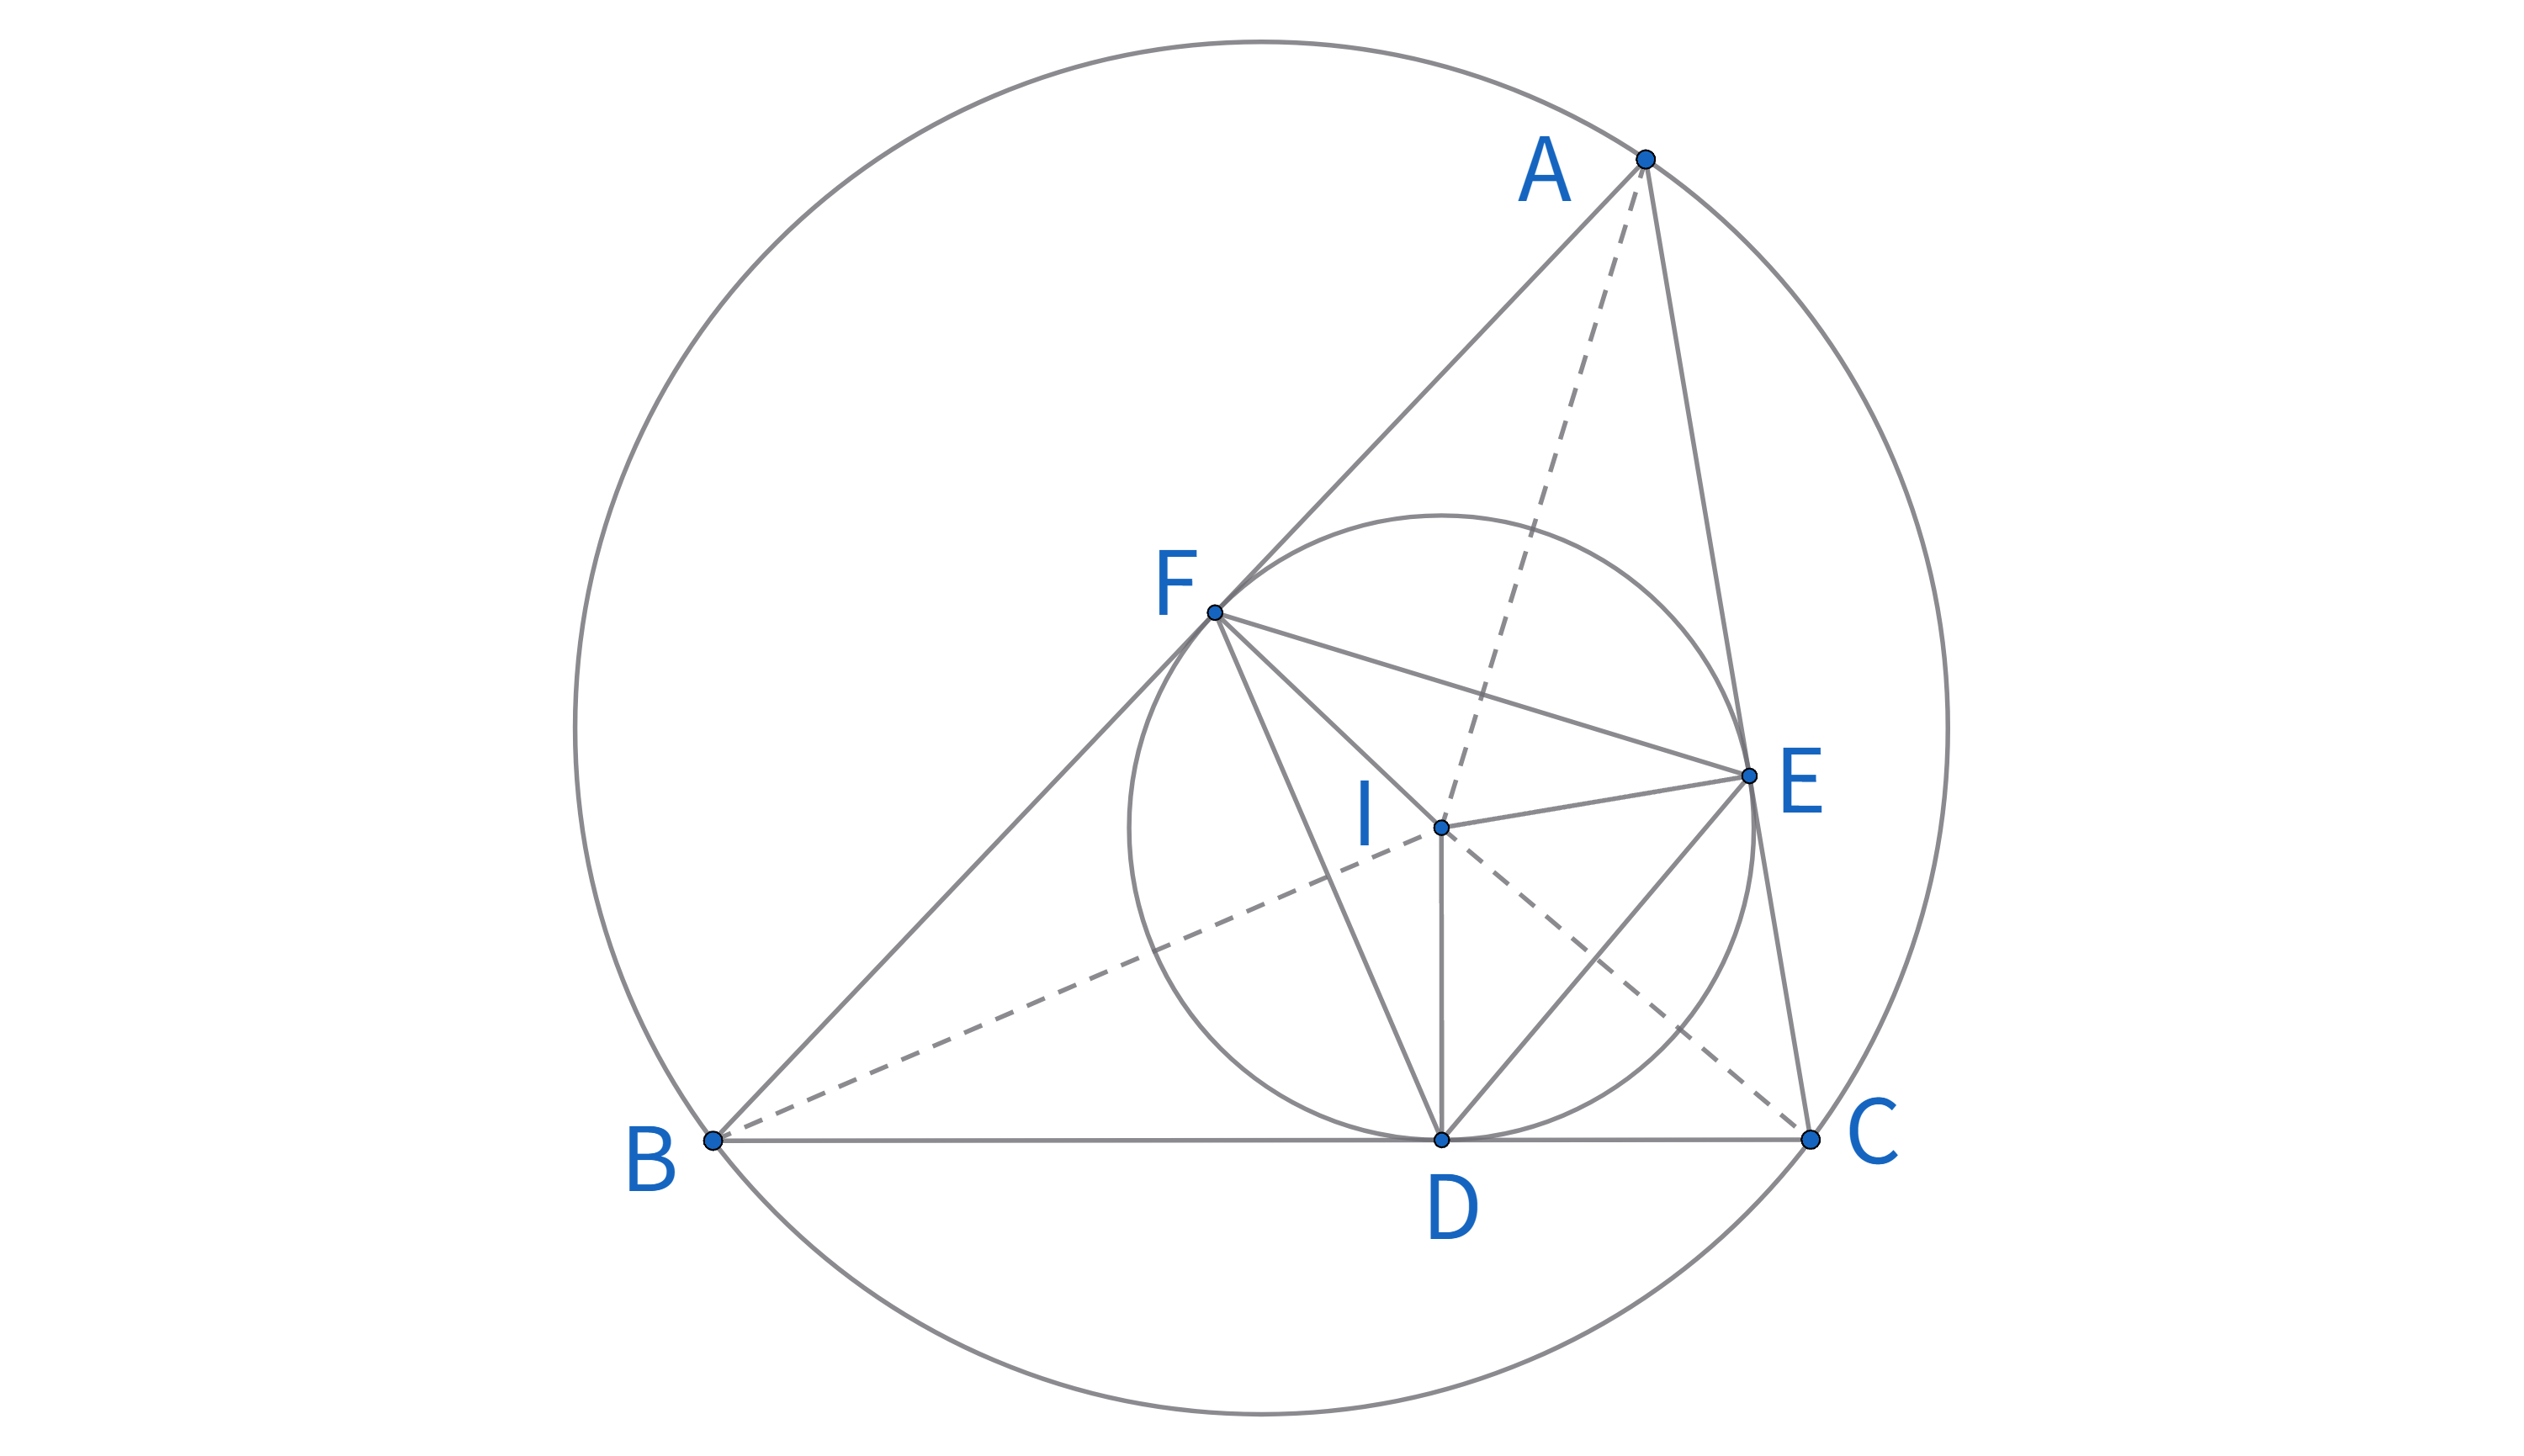
\includegraphics[width=0.7\linewidth]{figures/三角形五心/切点三角形.png}
%     \caption{切点三角形}
% \end{figure}


%--------------------------------------------------------------
\newpage
\section{垂心}
\begin{definition}[垂心]
    三角形三边上高线的交点称为三角形的垂心,通常使用H表示。
\end{definition}

\begin{figure}[H]
    \centering
    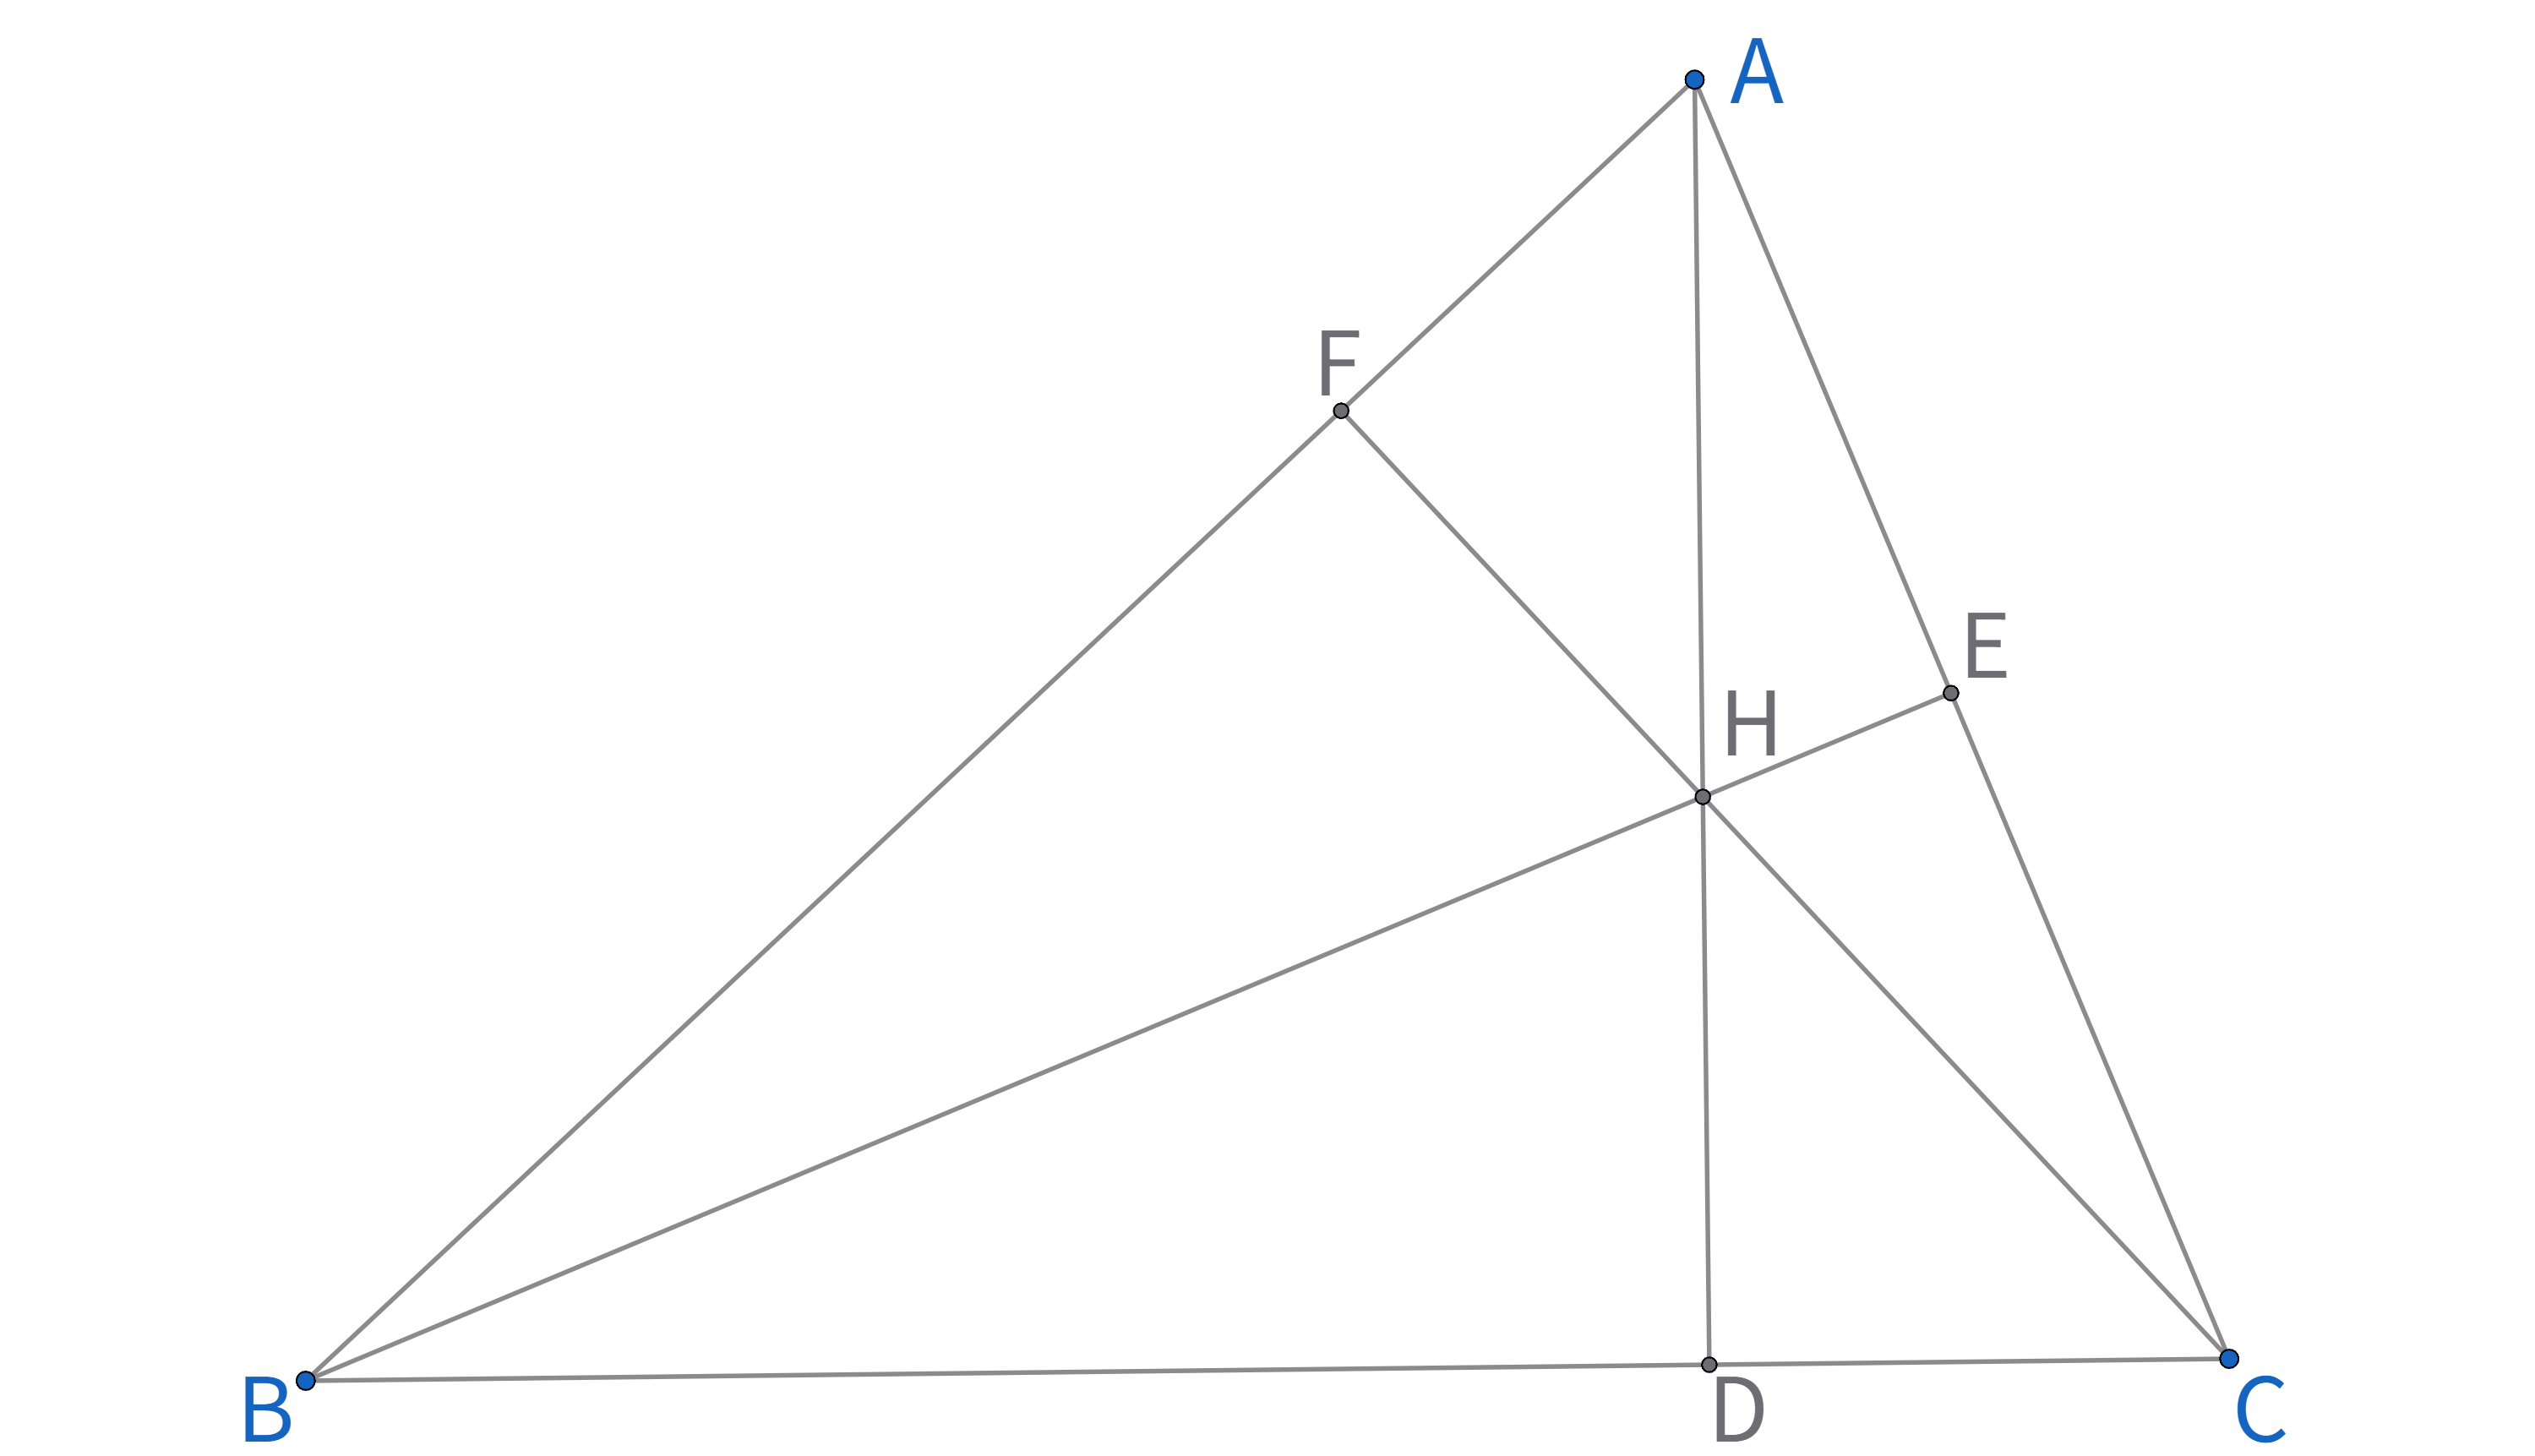
\includegraphics[width=0.8\linewidth]{figures/三角形五心/垂心.png}
    \caption{垂心}
\end{figure}

\begin{proposition}[垂心性质]
    三角形垂心具有如下性质。

    (1) 若H是三角形$\triangle ABC$的垂心,则
    $$\angle BHC = 180^\circ - A,\quad \angle AHC = 180^\circ - B,\quad \angle AHB =180^\circ - C.$$

    (2) 设$\triangle ABC$的外接圆半径为R,则
    $$AH=2R\cdot |\cos A|,\quad
    BH=2R\cdot |\cos B|,\quad
    CH=2R\cdot |\cos C|.$$

    (3) 锐角三角形的垂心在形内,直角三角形的垂心在直角顶点,钝角三角形的垂心在形外。

    (4) 若H为三角形$\triangle ABC$的垂心,则A、B、C、H四点中任意一点是其余三点构成的三角形的垂心,称A、B、C、H为垂心组。
\end{proposition}


\newpage
\subsection{垂足三角形}
\begin{proposition}[垂足三角形]
    设$\triangle DEF$ 是锐角$\triangle ABC$的垂足三角形,H是垂心,则:
    (1) $A, E, F, H$在以$AH$为直径的圆上。

    (2) $B, E, F, C$在以$BC$为直径的圆上。

    (3) $H$ 是 $\triangle DEF$的内心。
\end{proposition}
\begin{figure}[H]
    \centering
    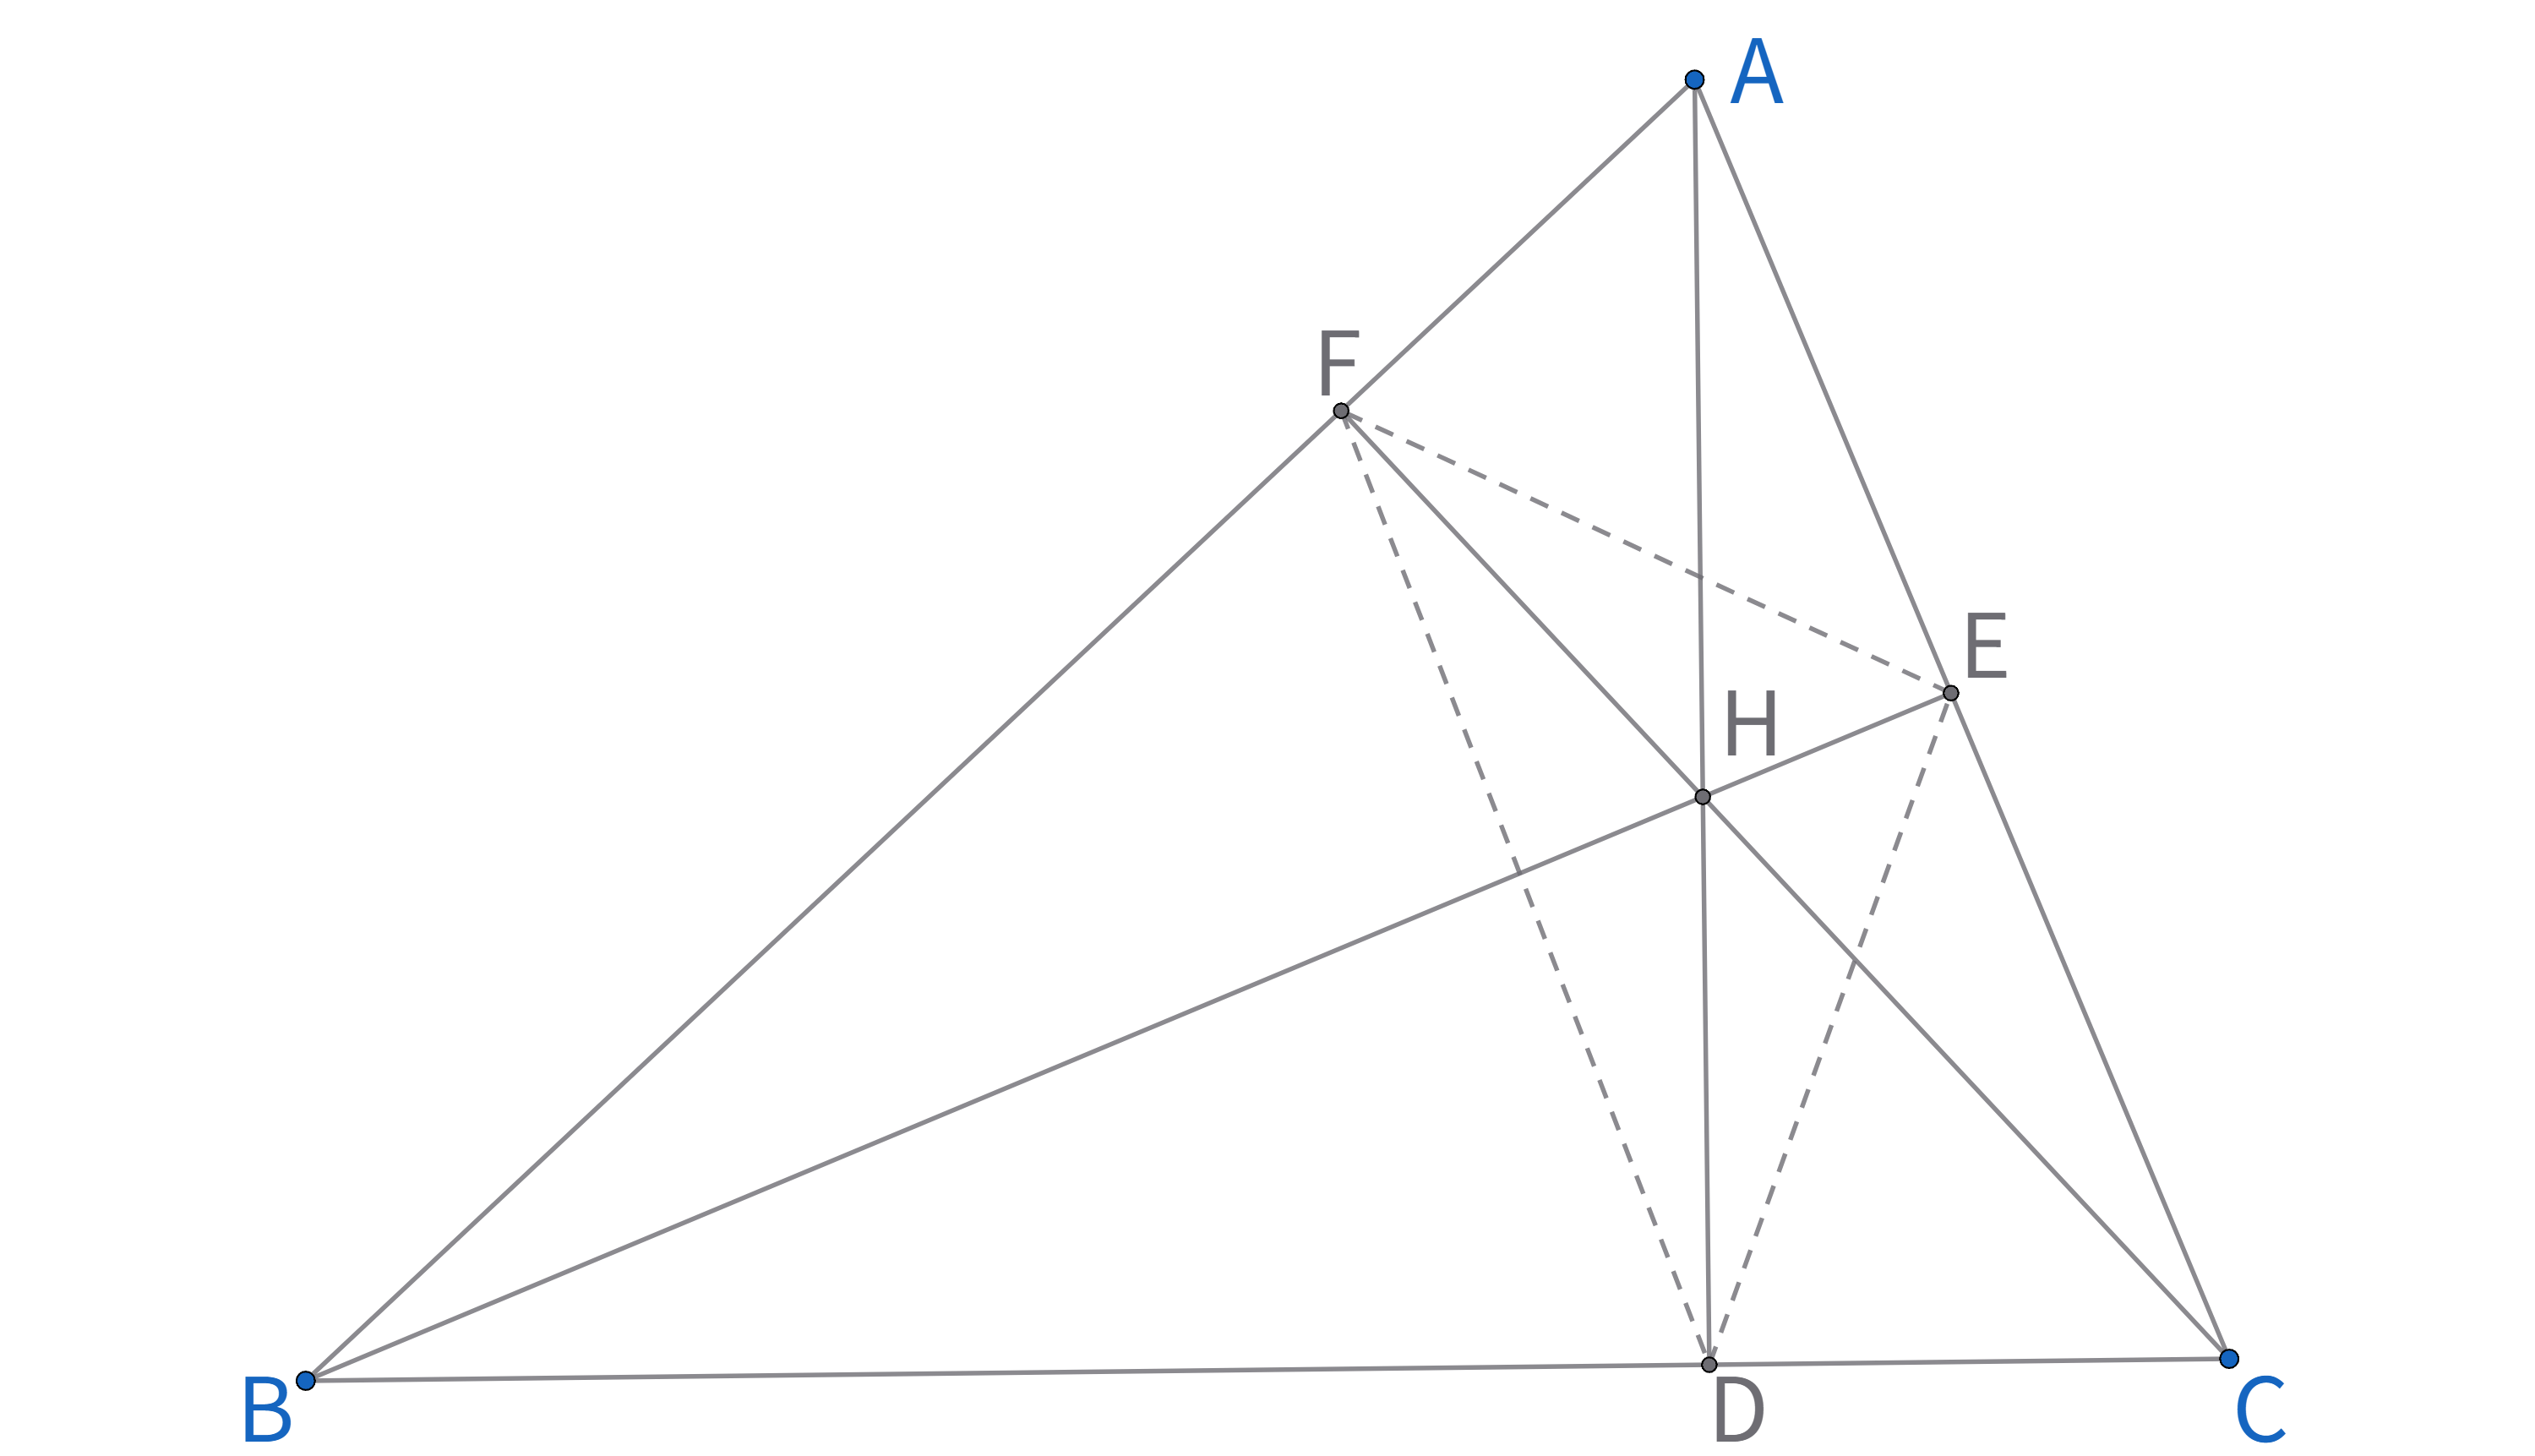
\includegraphics[width=0.8\linewidth]{figures/三角形五心/垂足三角形.png}
    \caption{垂足三角形}
\end{figure}

\begin{exercise}
    用$\triangle ABC$的三边边长,以及三顶角的三角函数表示下面的量。

    (1) 顶点与垂足连线段的长度,如$BD, CD$。

    (2) 垂心$H$到三边的距离,如$HD$。

    (3) 垂心$H$到三顶点的距离,如$HA$。

    (4) 两垂足连线段的长度,如$EF$。

    (5) 计算图中所有角的度数,如$\angle BAH, \angle AHF, \angle AEF, \angle FHE$。  
\end{exercise}




\newpage 
\subsection{垂心的对称性质}
\begin{figure}[H]
    \centering
    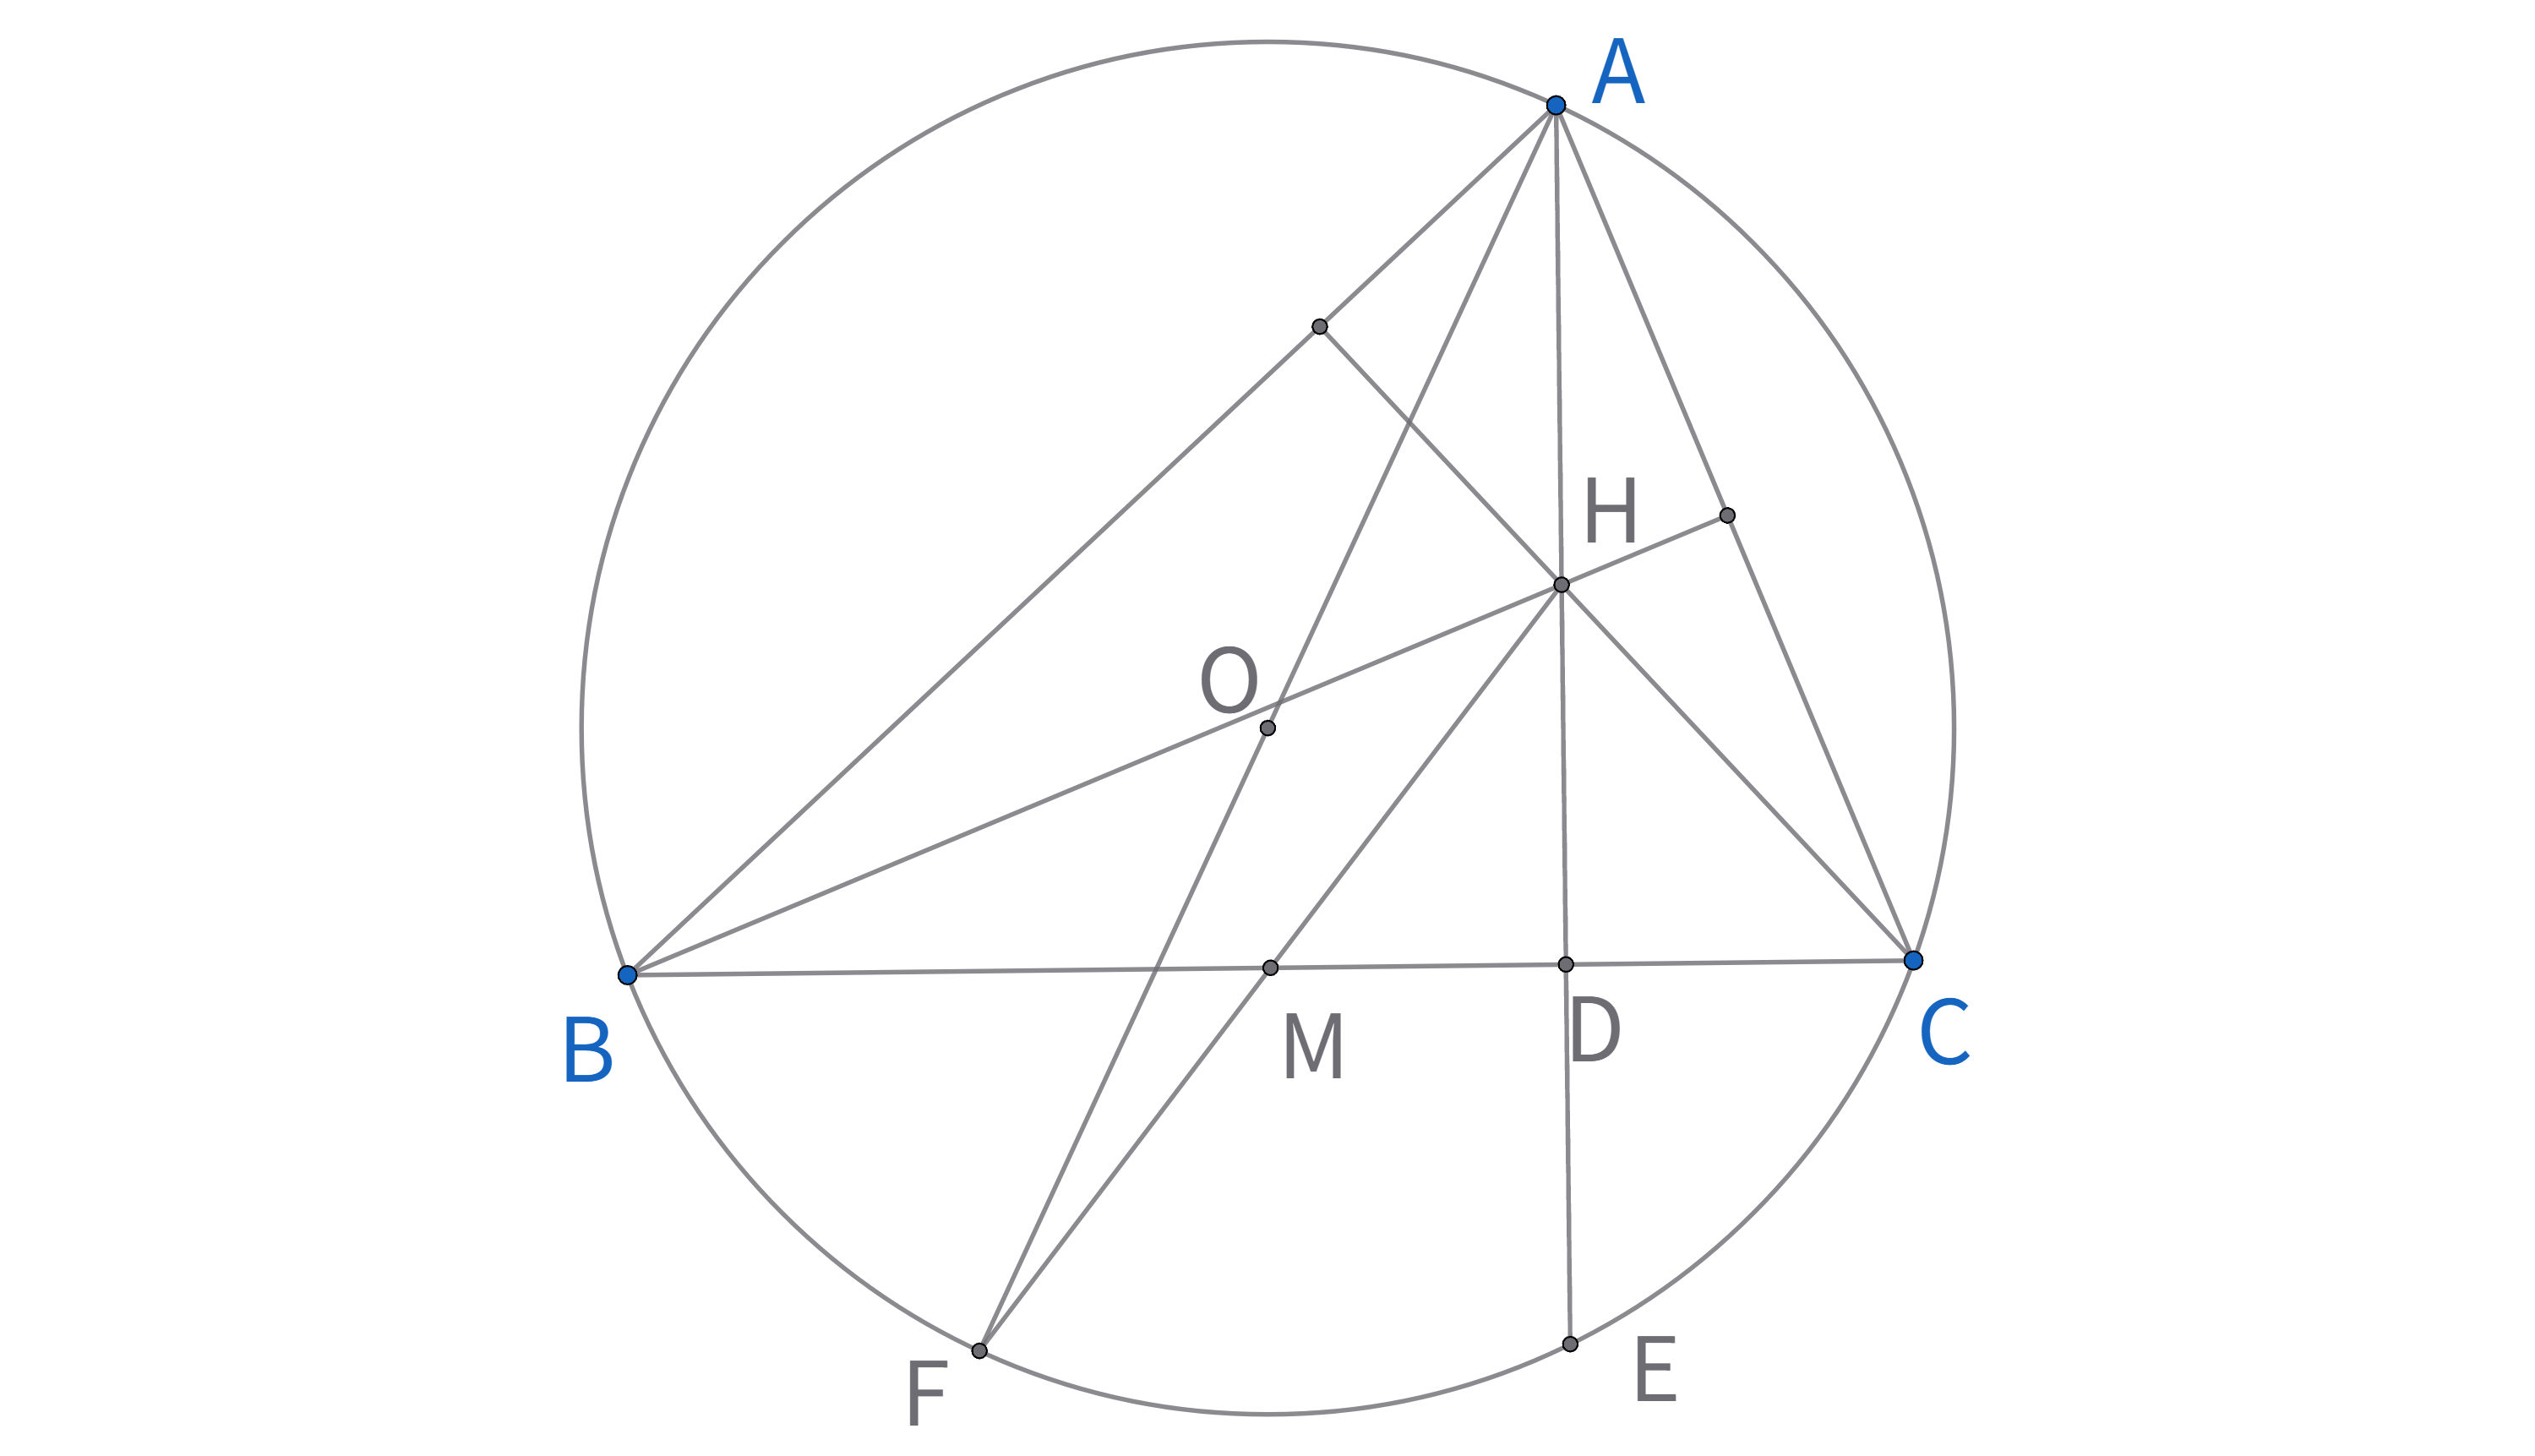
\includegraphics[width=0.8\linewidth]{figures/三角形五心/垂心的对称性质.png}
    \caption{垂心性质}
\end{figure}

\begin{theorem}[垂心的对称性质]
    设$H$是$\triangle ABC$的垂心,设$E$ 是 $H$ 关于$BC$的对称点, $F$ 是$H$ 关于 $BC$中点$M$的对称点。

    (1) $E$在$\triangle ABC$的外接圆$O$上。


    (2) $F$在$\triangle ABC$的外接圆$O$上。

    (3) $A, O, F$ 三点共线。

    (4) (卡诺定理) 顶点到垂心距离是外心到对边距离的2倍,即$AH = 2OM.$
   
    (5) H是外心O关于$\triangle ABC$的等角共轭点,即
    $$\angle BAO = \angle CAH, \quad 
    \angle ACO = \angle BCH, \quad 
    \angle CBO = \angle ABH.$$
\end{theorem}

% \begin{figure}[H]
%     \centering
%     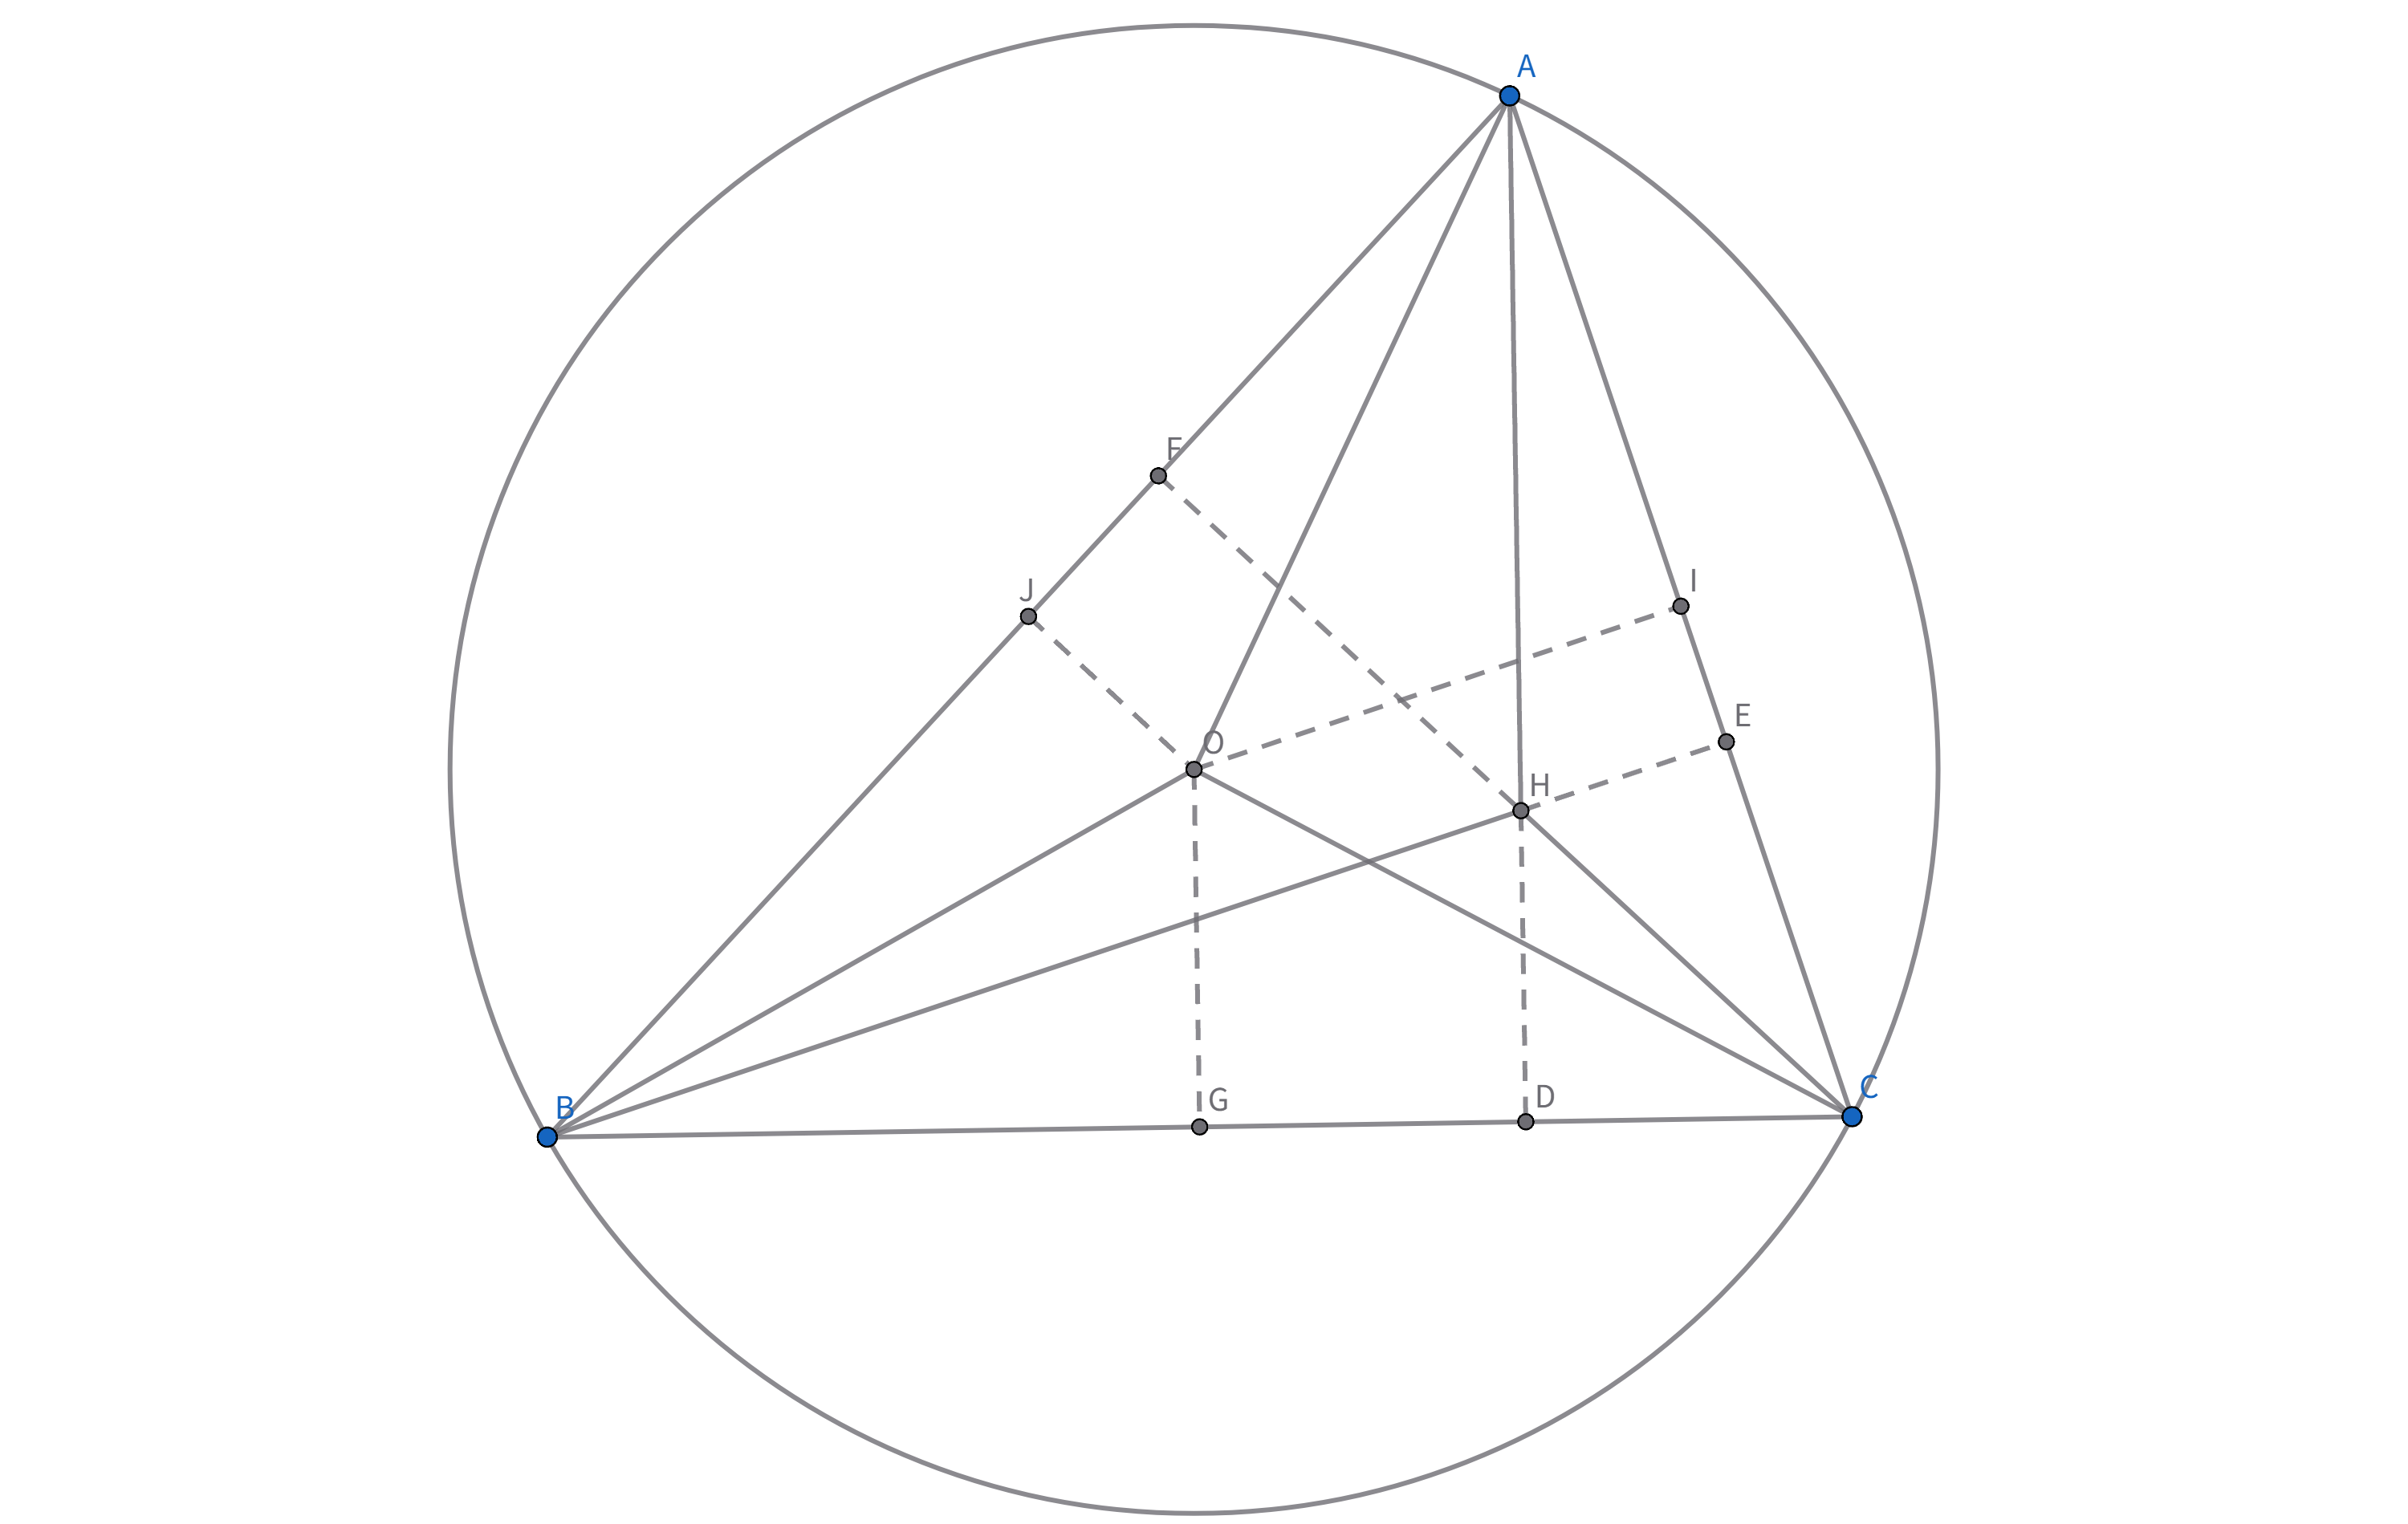
\includegraphics[width=0.5\linewidth]{figures/三角形五心/外心垂心等角共轭.png}
%     \caption{外心垂心等角共轭}
% \end{figure}


%-----------------------------------------------------------------------------------------
\newpage
\section{重心}
\begin{definition}[重心]
    三角形三条中线的交点称为三角形的重心,通常使用G表示。
\end{definition}

\begin{figure}[H]
    \centering
    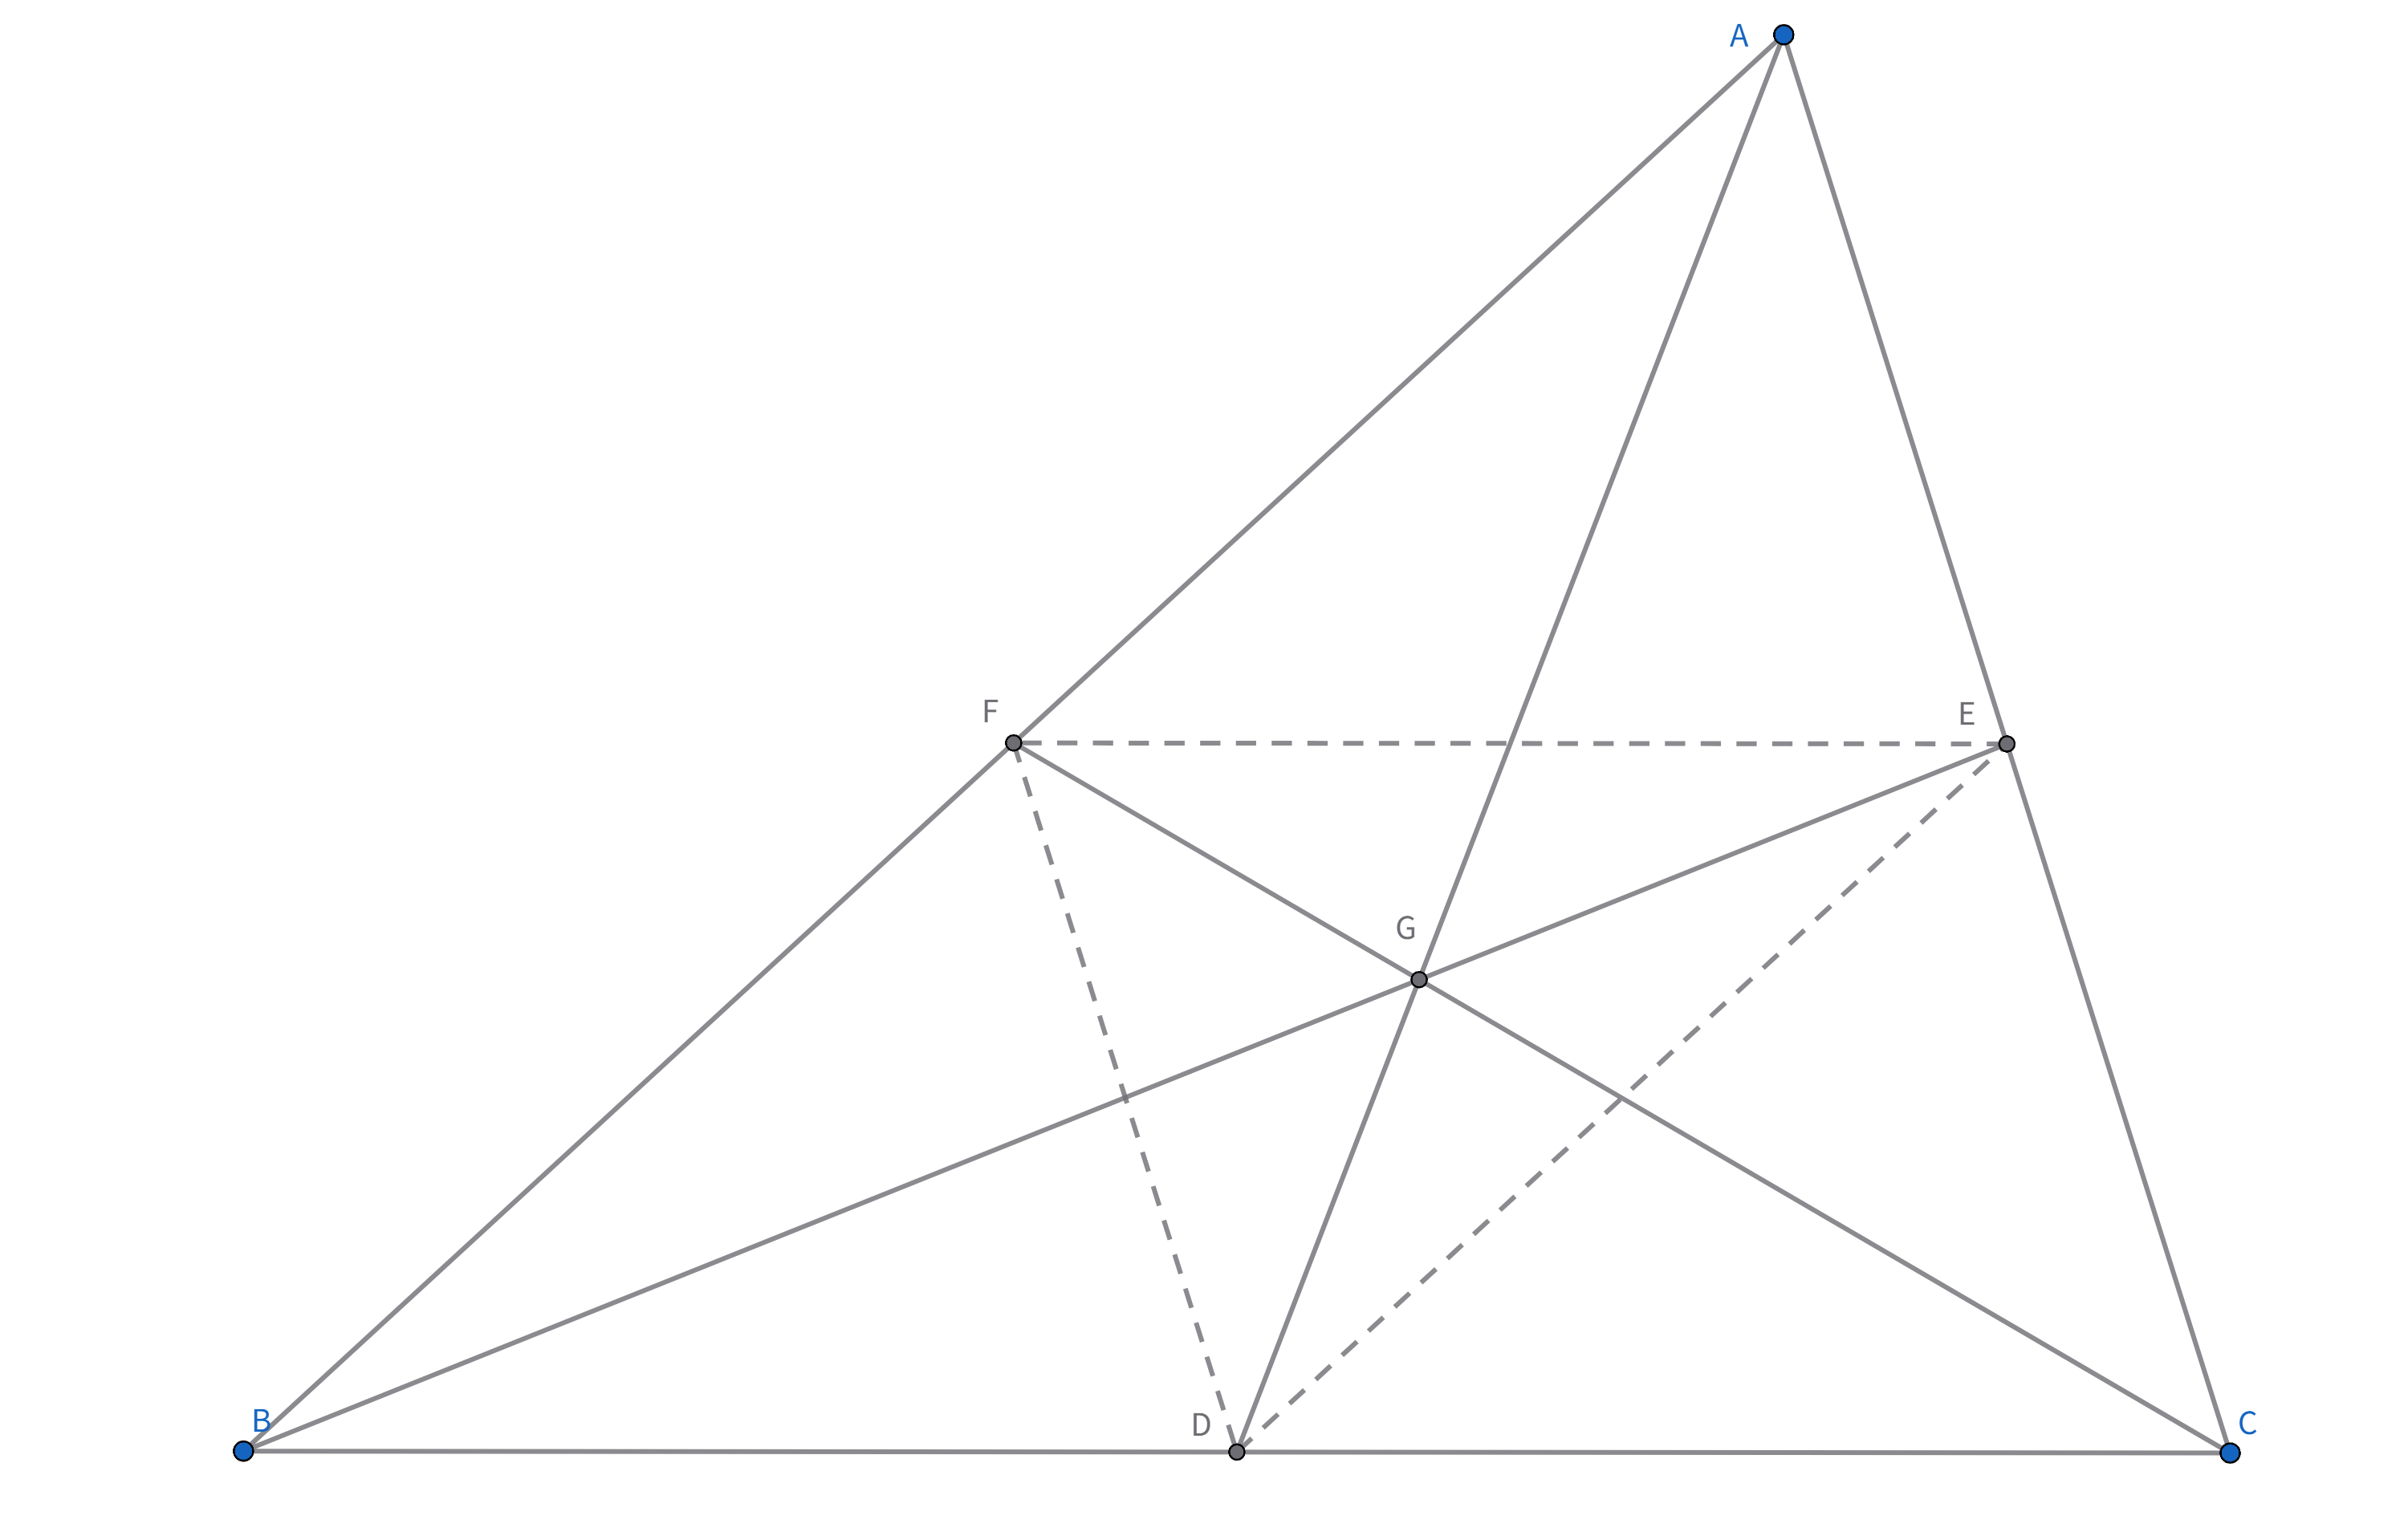
\includegraphics[width=0.8\linewidth]{figures/重心.png}
    \caption{重心}
\end{figure}

\begin{proposition}[重心性质]
    三角形重心具有如下性质。
    
    (1) 重心G为三条中线的三等分点,满足
    $$AG=2GD,\quad 
    BG=2GE,\quad
    CG=2GF.$$

    (2) 三边与重心组成的三角形面积相等,即
    $$S_{\triangle ABG} = S_{\triangle BCG}=S_{\triangle CAG}.$$

    (3) $\triangle ABC \sim \triangle DEF$,且相似比为2.
\end{proposition}
%-------------------------------------------------------------
\begin{exercise}
    证明:$2AD^2=AB^2+AC^2-\frac{1}{2}BC^2.$
\end{exercise}
\begin{exercise}
    证明:在平面直角坐标系中,重心$G$的坐标可以表示为三顶点坐标的算术平均值。
\end{exercise}


\newpage
\section{旁心}
\begin{definition}[旁心]
    与三角形一边外侧相切,又与另两边的延长线相切的圆叫做三角形的旁切圆,通常用J,或者$I_a,I_b,I_c$表示。    
\end{definition}

\begin{figure}[H]
    \centering
    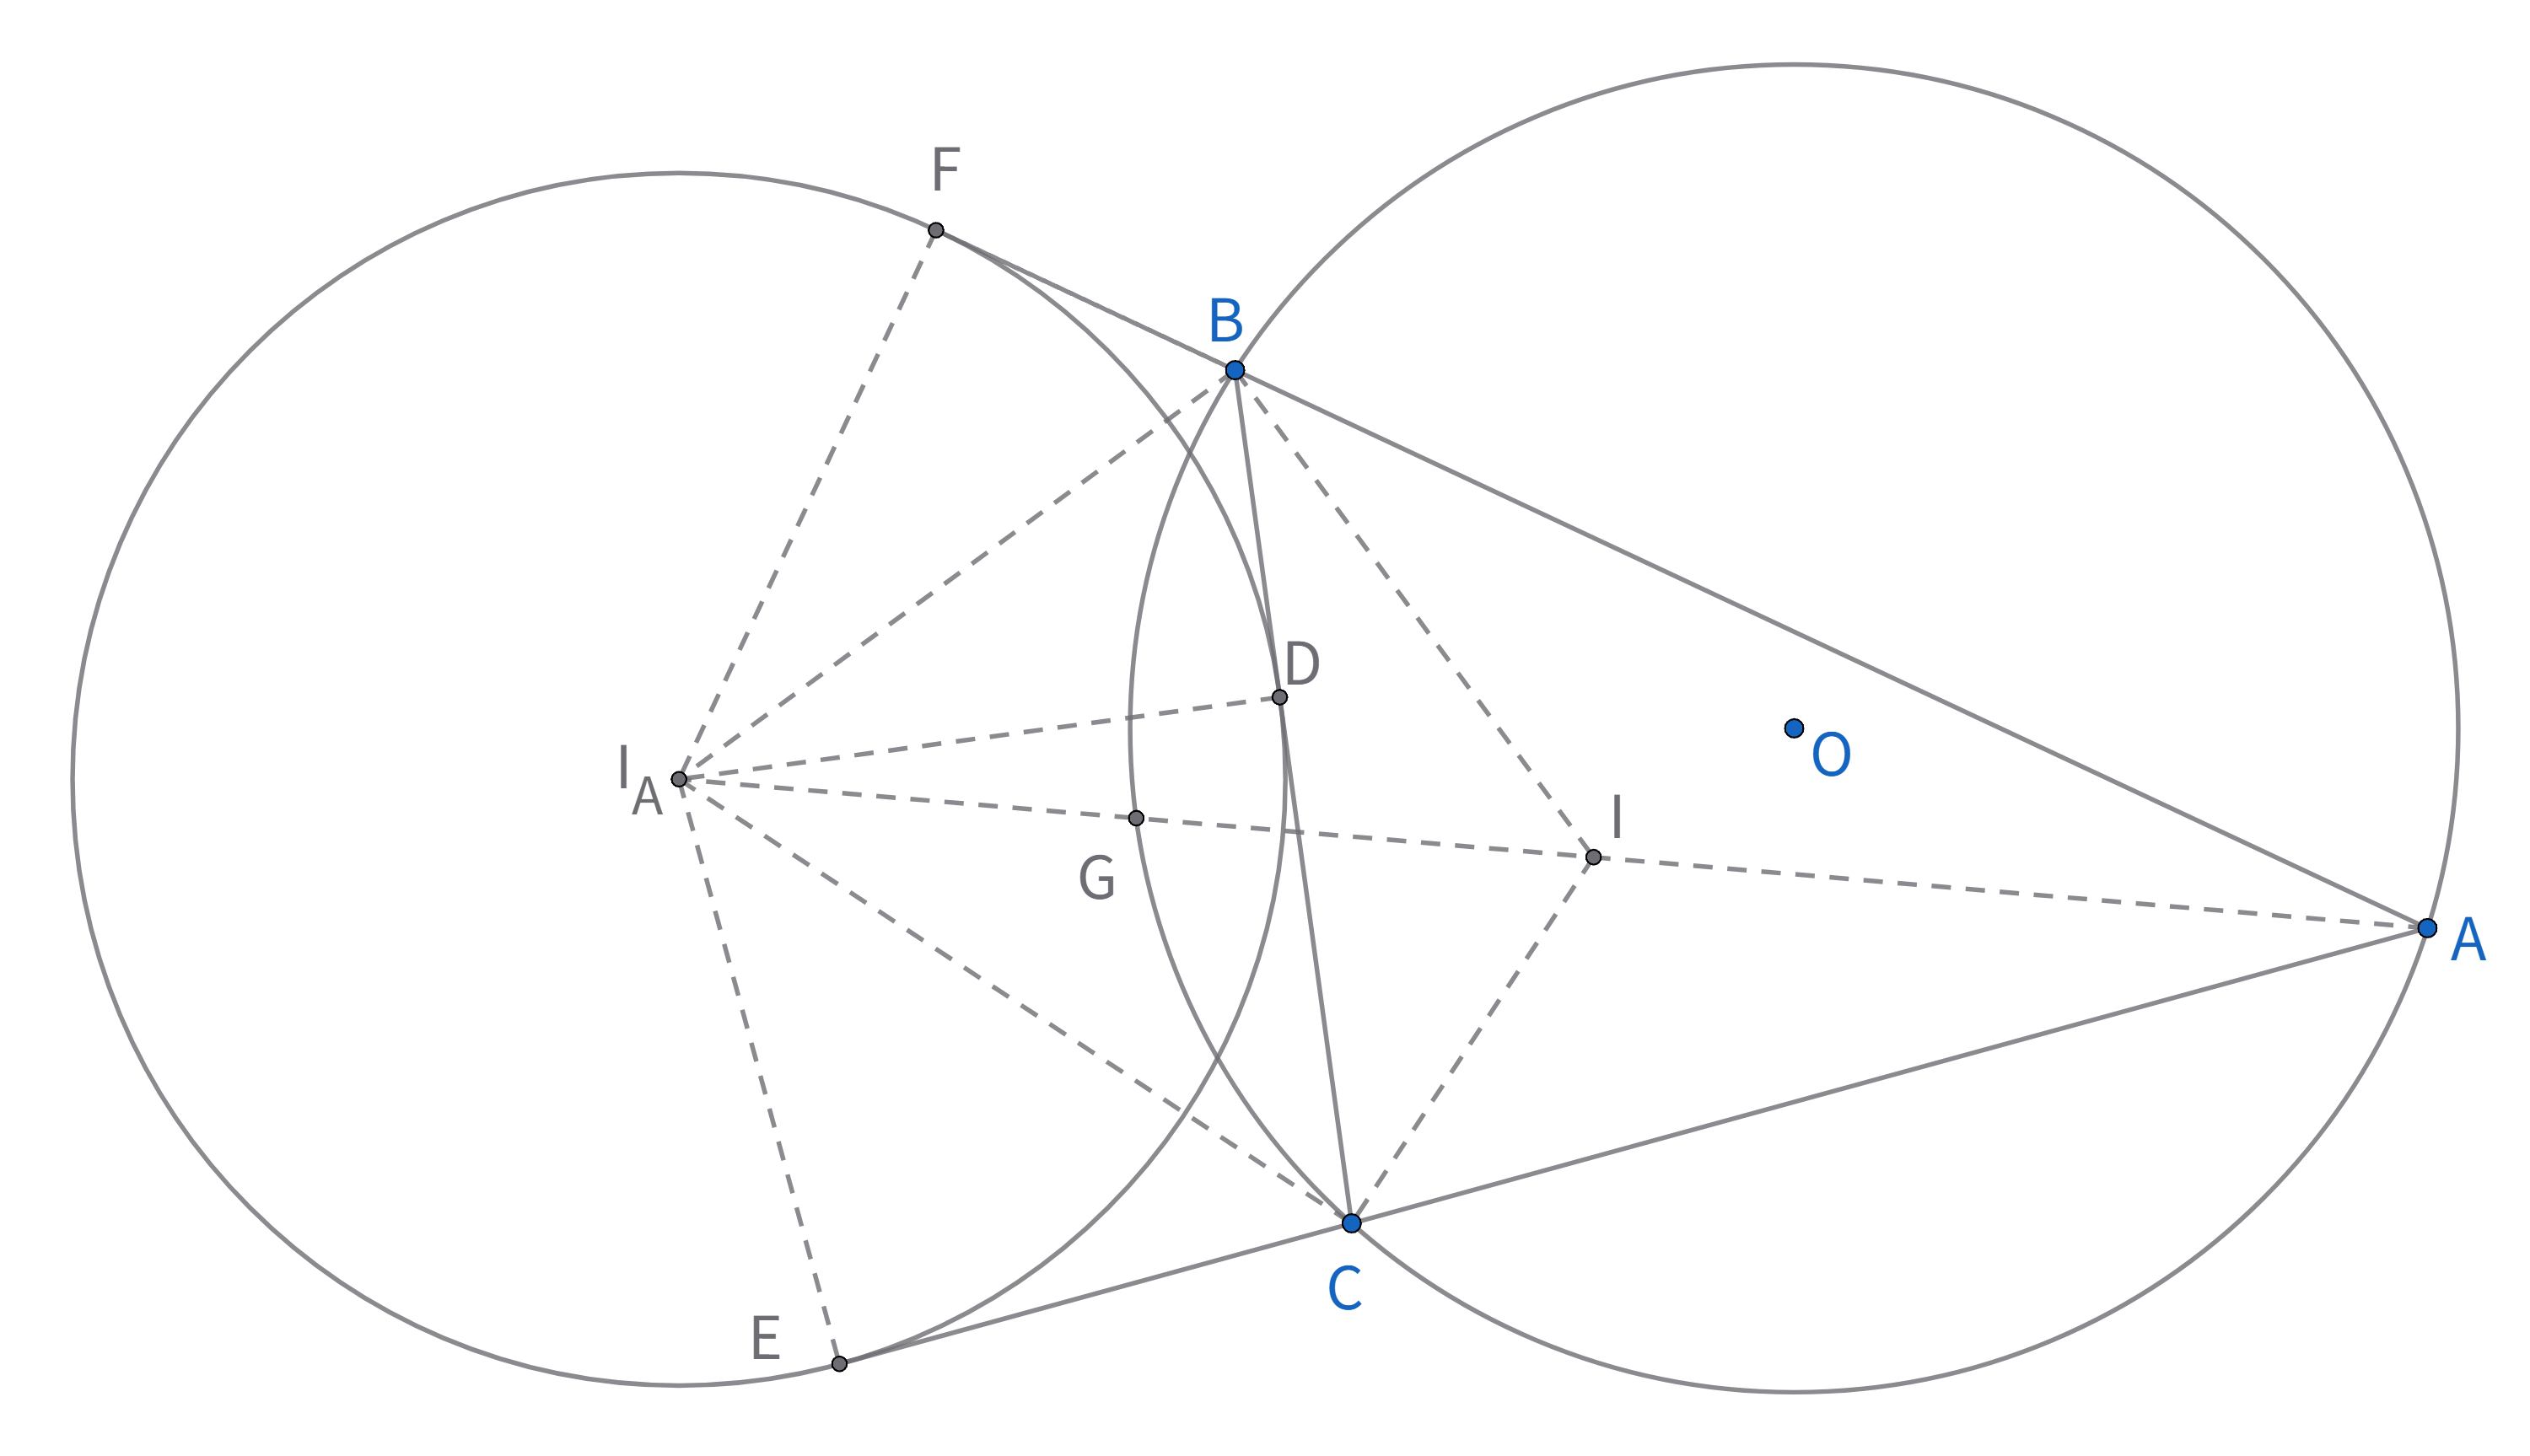
\includegraphics[width=0.6\linewidth]{figures/三角形五心/旁心.png}
    \caption{旁心}
\end{figure}


\begin{proposition}[旁心性质]
    三角形旁心具有如下性质。
    
    (1) 旁心是三角形一内角平分线及其他两角外角平分线的交点。

    (2) 旁心到三角形三边的距离相等。

    (3) $\angle I_ABC = 90^\circ - \frac{1}{2}B, \angle I_ACB = 90^\circ - \frac{1}{2}C, \angle BI_AC=90 - \frac{1}{2}A.$

    (4) $IB\perp BI_A, \quad IC\perp CI_A.$
\end{proposition}

\begin{proposition}[切线长性质]
    设D、E、F分别为旁切圆$I_A$在BC、CA、AB上的切点,则
    $$
    \begin{aligned}
    AE&=AF= s = \frac{1}{2}(a+b+c),\\
    BF&=BD=s - c =\frac{1}{2}(a+b-c),\\
    CD&=CE=s - b= \frac{1}{2}(a+c-b).
    \end{aligned}
    $$
\end{proposition}


\newpage 
\subsection{鸡爪定理}
\begin{theorem}[鸡爪定理]
    对平面内任意$\triangle ABC$,$I,J$ 分别为其内心和A-旁心,设$AI$延长线与圆$O$相交于$D$,则D为$\overset{{\frown}}{BC}$的中点,$IJ$的中点,并且为$IBJC$外接圆的圆心。
\end{theorem}

\begin{figure}[H]
    \centering
    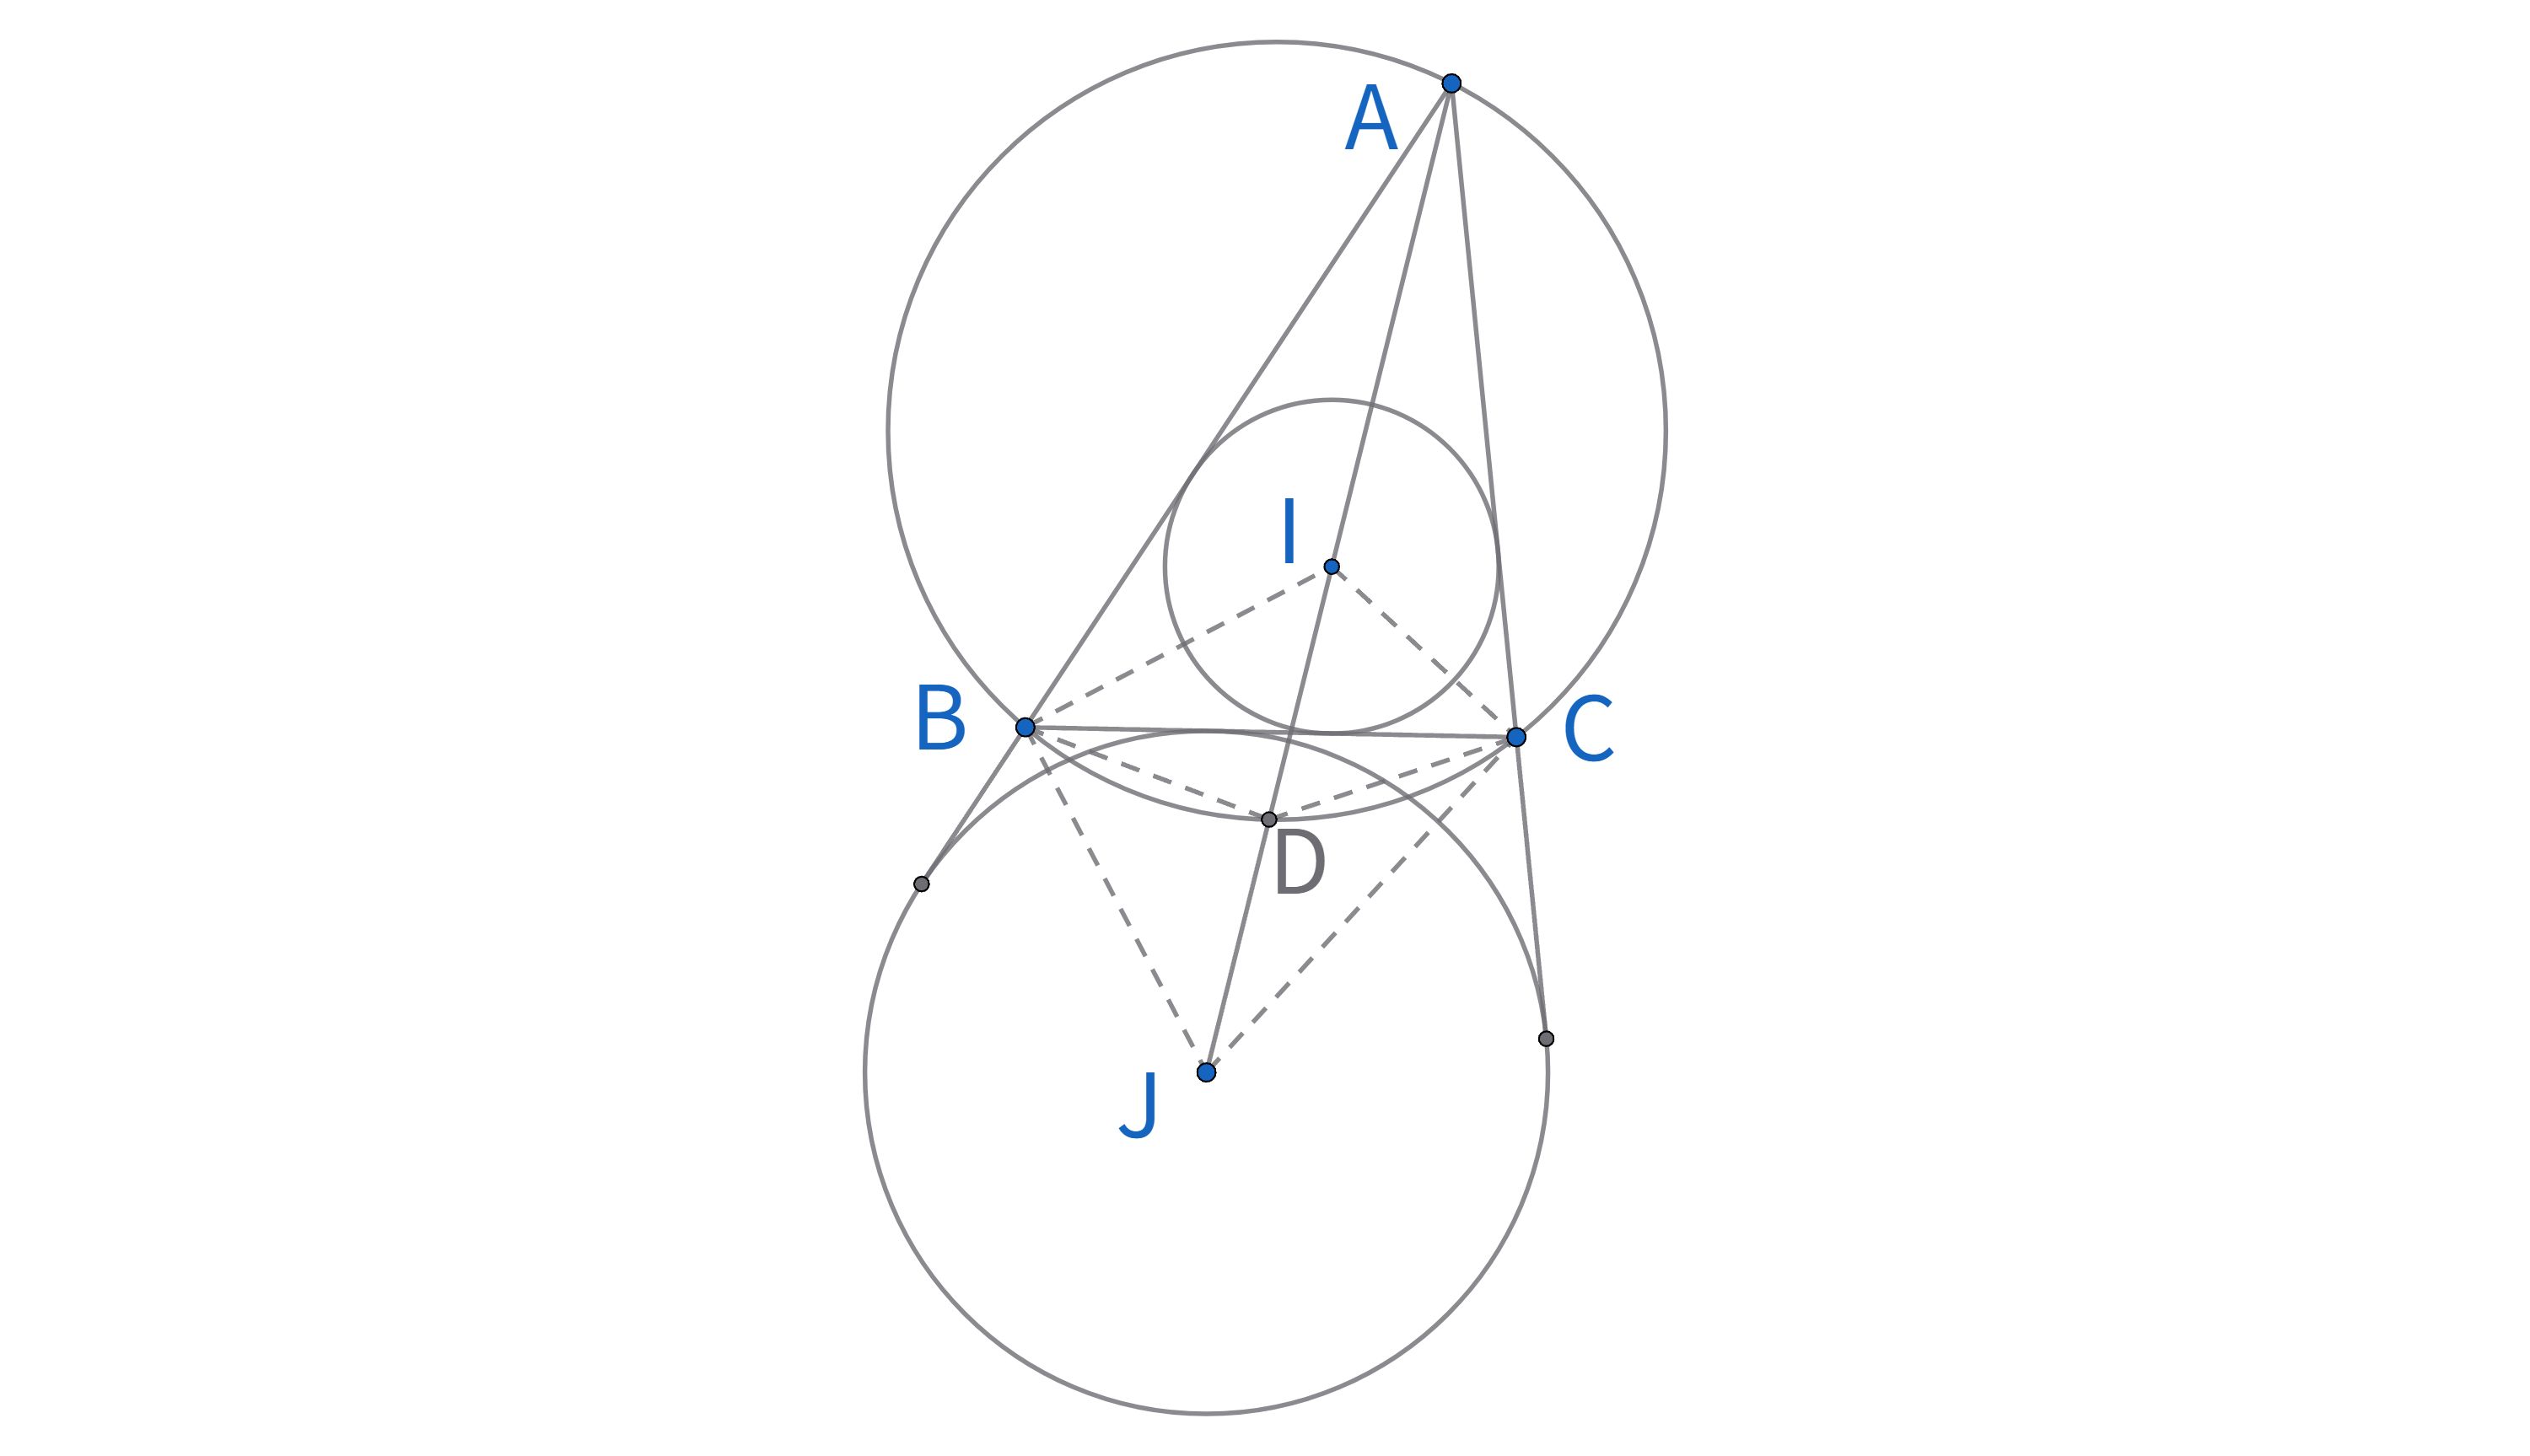
\includegraphics[width=\linewidth]{figures/三角形五心/鸡爪定理2.png}
    \caption{鸡爪定理}
\end{figure}

\begin{exercise}
    计算$\angle BIJ, \angle CIJ, \angle IBD, \angle ICD$。
\end{exercise}
\begin{exercise}
    计算$IJ$。
\end{exercise}
\begin{exercise}[旁切圆半径]
    证明:A-旁切圆的半径为$r_a = \frac{s}{s-a}r.$
\end{exercise}


\begin{exercise}
    设 $\triangle ABC$ 的内切圆和 $A$-旁切圆在 $BC$ 上的切点分别是 $D, X$。证明:$BX = CD, BD = CX$。
\end{exercise}



\newpage 
\subsection{旁心三角形}
\begin{proposition}[旁心三角形]
    对平面内任意$\triangle ABC$,$I, I_A,I_B,I_C$ 为其内心和三旁心。则$I$是旁心所构成$\triangle I_AI_BI_C$ 的垂心,$\triangle ABC$是其垂足三角形。
\end{proposition}

\begin{figure}[H]
    \centering
    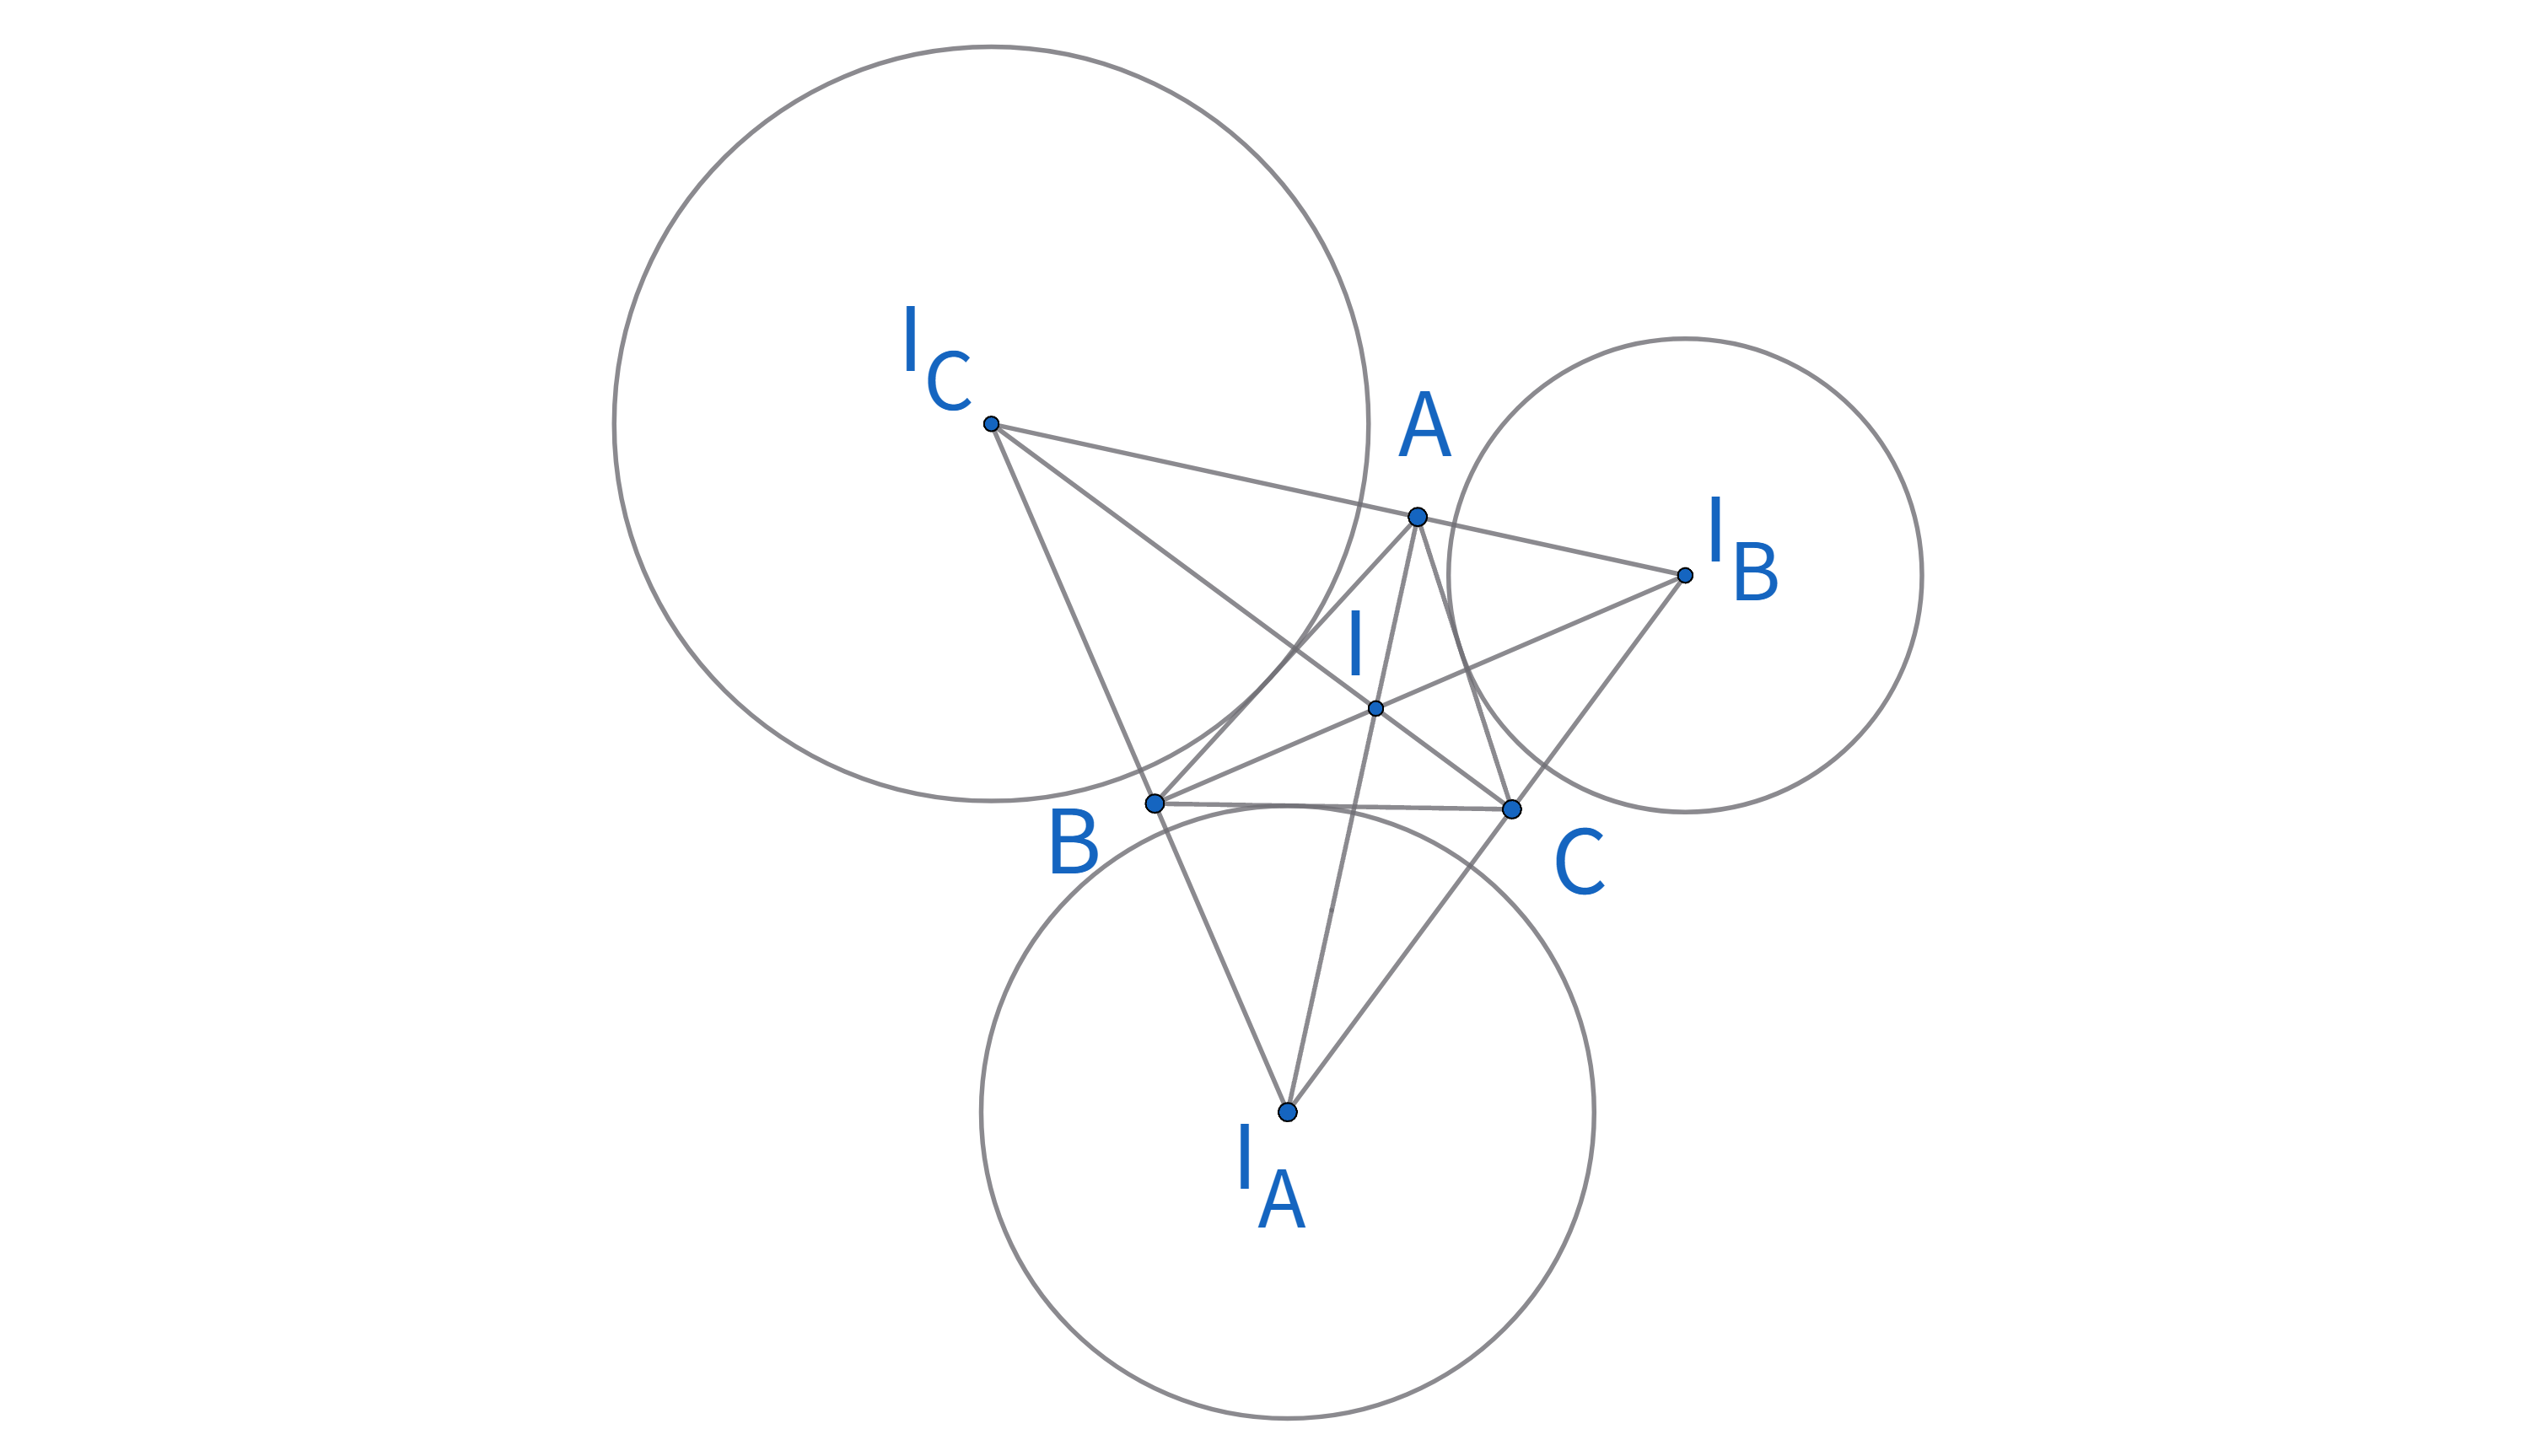
\includegraphics[width=\linewidth]{figures/三角形五心/旁心三角形.png}
    \caption{旁心三角形}
\end{figure}




